%!TEX root = main.tex


\section{Variables and Probability Models}\label{sec:vague_variables}

\subsection{Probability gap models - executive summary}

Just like everybody else, we consider a probability model to be a probability space $(\Omega,\sigalg{F},\mu)$ along with a collection of random variables. However, if I want to use probabilistic models to support decision making, I need something different to a probability model; I need function from options to probability models. For example, suppose I have two options $A=\{0,1\}$, and I want to compare these options based on what I expect to happen if I choose them. If I choose option $0$, then I can (perhaps) represent my expectations about the consequences with one probability model, and if I choose option $1$ I can represent my expectations about the consequences with a different probability model. I can compare the two consequences, then decide which option seems to be better. To make this comparison, I need to have a function from elements of $A$ to probability models. A function that takes elements of some set as inputs (which may or may not be decisions) and returns probability models is a \emph{probability gap model}, and the set of inputs it accepts is a \emph{probability gap}.

We are particularly interested in probability gap models where the consequences of all inputs share some marginal or conditional probabilities. The simplest example of a model like this can be represented by a probability distribution $\prob{P}^{\RV{X}}$ for some variable $\RV{X}:\Omega\to X$. Such a probability distribution is consistent with many base measures on the sample space $\Omega$, and so we can define a probability gap model $\prob{P}$ that takes inputs in $A$ and maps them to base measures with the particular property that the marginal distribution of $\RV{X}$ is equal to $\prob{P}^{\RV{X}}$ for any base measure in the image $\prob{P}(A)$. Just like everybody else, we don't often explicitly define the sample space, and we don't regard the particular choice of base measure as a particularly interesting question. Nonetheless, we begin by investigating this kind of probability gap model because it raises an important issue: not every probability distribution over $X$ is a \emph{valid} marginal probability. In particular, we need $\prob{P}^{\RV{X}}$ to assign probability 0 to outcomes that are mathematically impossible according to the definition of $\RV{X}$ to ensure that there is some base measure that features $\prob{P}^{\RV{X}}$ as a marginal. We call probability gap models represented by probability distributions \emph{order 0 probability gap models}.

More interesting probability gap models are those that can be represented by conditional probabilities $\prob{P}^{\RV{Y}|\RV{X}}$ or pairs of conditional probabilities $\{\prob{P}^{\RV{X}|\RV{W}},\prob{P}^{\RV{Z}|\RV{WXY}}\}$, which we call \emph{order 1} and \emph{order 2} models respectively. Probability gaps in order 2 models correspond to decision functions in some kinds of decision problem, which is the reason we wanted to investigate probability gap models in the first place. These too need to be valid, and we define conditions for validity and prove that they are sufficient to ensure that models represented by conditional probabilities can in fact be mapped to base measures on the sample space.

A conditional independence statement in a probability gap model means that the corresponding conditional independence statement holds for all base measures in the range of the function defined by the model. It is possible to deduce conditional independences from ``independences'' in the conditional probabilities that we use to represent these models, and conditional independences can imply the existence of conditional probabilities with certain independence properties.

We can consider causal Bayesian networks to represent order 2 probability gap models. That is, a causal Bayesian network represents a function $\prob{P}$ that take inserts from some set $A$ and returns probability models, and it does so in such a way that we can identify conditional probabilities $\{\prob{P}^{\RV{X}|\RV{W}},\prob{P}^{\RV{Z}|\RV{WXY}}\}$ shared by all models in the codomain. The observational distribution is the value of $\prob{P}(\text{obs})$ for some element $\text{obs}\in A$, and interventional distributions are found by choosing other inserts. We believe that this definition is improves on the standard definition in two ways: firstly, interventional probabilities according to the standard definition fail to exist in some situations, while we offer conditions under which an order 2 model is valid that guarantee existence. Secondly, we make explicit the fact that there may be many functions $\prob{P},\prob{P}',...$ which may differ in important ways that all map to the same $\prob{P}(\text{obs})$.


\subsection{Probability distributions, Markov kernels and string diagrams}

We make extensive use of probability theory, and the following is a brief introduction to the string diagram notation we use for probabilistic reasoning. This notation comes from the study of Markov categories. Markov categories are abstract categories that represent models of the flow of information. We can form Markov categories from collections of sets -- for example, discrete sets or standard measurable sets -- along with the Markov kernel product as the composition operation. Markov categories come equipped with a graphical language of \emph{string diagrams}, and a coherence theorem which states that calid proofs using string diagrams correspond to valid theorems in \emph{any} Markov category \citep{selinger_survey_2010}. More comprehensive introductions to Markov categories can be found in \citet{fritz_synthetic_2020,cho_disintegration_2019}. Thus, while we limit ourselves to discrete sets in this paper, any derivation that uses only string diagrams is more broadly appliccable.

We say, given a variable $\RV{X}:\Omega\to X$, a probability distribution $\prob{P}^{\RV{X}}$ is a probability measure on $(X,\sigalg{X})$. Recall that a probability measure is a $\sigma$-additive function $\prob{P}^{\RV{X}}:\sigalg{X}\to [0,1]$ such that $\prob{P}^{\RV{X}}(\emptyset)=0$ and $\prob{P}^{\RV{X}}(X)=1$. Given a second variable $\RV{Y}:\Omega\to Y$, a conditional probability $\prob{Q}^{\RV{X}|\RV{Y}}$ is a Markov kernel $\prob{Q}^{\RV{X}|\RV{Y}}:X\kto Y$which is a map $Y\times \sigalg{X}\to [0,1]$ such that

\begin{enumerate}
	\item $y\mapsto \prob{Q}^{\RV{X}|\RV{Y}}(A|y)$ is $\sigalg{B}$-measurable for all $A\in \sigalg{X}$
	\item $A\mapsto \prob{Q}^{\RV{X}|\RV{Y}}{K}(A|y)$ is a probability measure on $(X,\sigalg{X})$ for all $y\in Y$
\end{enumerate}

In the context of discrete sets, a probability distribution can be defined as a vector, and a Markov kernel a matrix.

\begin{definition}[Probability distribution (discrete sets)]
A probability distribution $\prob{P}$ on a discrete set $X$ is a vector $(\prob{P}(x))_{x\in X}\in [0,1]^{|X|}$ such that $\sum_{x\in X} \prob{P}(x) = 1$. For $A\subset X$, define $\prob{P}(A)=\sum_{x\in A} P(x)$.
\end{definition}

\begin{definition}[Markov kernel (discrete sets)]
A Markov kernel $\prob{K}:X\kto Y$ is a matrix $(\prob{K}(y|x))_{x\in X,y\in Y}\in [0,1]^{|X||Y|}$ such that $\sum_{y\in Y} \prob{K}(y|x)=1$ for all $x\in X$. For $B\subset Y$ define $\prob{K}(B|x)=\sum_{y\in B}\prob{K}(y|x)$.
\end{definition}

In the graphical language, Markov kernels are drawn as boxes with input and output wires, and probability measures (which are kernels with the domain $\{*\}$) are represented by triangles:

\begin{align}
\kernel{K}&:=\begin{tikzpicture}[baseline={([yshift=-.5ex]current bounding box.center)}]
	\path (0,0) node (A) {}
	++ (0.5,0) node[kernel] (K) {$\kernel{K}$}
	++ (0.5,0) node (B) {};
	\draw (A) -- (K) -- (B);
\end{tikzpicture}\\
\kernel{P}&:= \begin{tikzpicture}[baseline={([yshift=-.5ex]current bounding box.center)}]
	\path (0,0) node[dist] (K) {$\kernel{P}$}
	++ (0.5,0) node (B) {};
	\draw (K) -- (B);
\end{tikzpicture}
\end{align}

Two Markov kernels $\kernel{L}:X\kto Y$ and $\kernel{M}:Y\kto Z$ have a product $\kernel{L}\kernel{M}:X\kto Z$, given in the discrete case by the matrix product $ \kernel{L}\kernel{M}(z|x) = \sum_{y\in Y} \kernel{M}(z|y)\kernel{L}(y|x)$. Graphically, we represent products between compatible Markov kernels by joining wires together:

\begin{align}
	\kernel{L}\kernel{M}:= \begin{tikzpicture}[baseline={([yshift=-.5ex]current bounding box.center)}]
	\path (0,0) node (A) {$X$}
	++ (0.5,0) node[kernel] (K) {$\kernel{K}$}
	++ (0.7,0) node[kernel] (M) {$\kernel{M}$}
	++ (0.5,0) node (B) {$Z$};
	\draw (A) -- (K) -- (M) -- (B);
\end{tikzpicture}
\end{align}

The Cartesian product $X\times Y:=\{(x,y)|x\in X, y\in Y\}$. Given kernels $\kernel{K}:W\kto Y$ and $\kernel{L}:X\kto Z$, the tensor product $\kernel{K}\otimes\kernel{L}:W\times X\kto Y\times Z$ given by $(\kernel{K}\otimes\kernel{L})(y,z|w,x):=K(y|w) L(z|x)$. The tensor product is graphically represeted by drawing kernels in parallel:

\begin{align}
	\kernel{K}\otimes \kernel{L}&:=\begin{tikzpicture}[baseline={([yshift=-.5ex]current bounding box.center)}]
	\path (0,0) node (A) {$W$}
	++ (0.5,0) node[kernel] (K) {$\kernel{K}$}
	++ (0.5,0) node (B) {$Y$};
	\path (0,-0.5) node (C) {$X$}
	++ (0.5,0) node[kernel] (L) {$\kernel{L}$}
	++ (0.5,0) node (D) {$Z$};
	\draw (A) -- (K) -- (B);
	\draw (C) -- (L) -- (D);
\end{tikzpicture}
\end{align}

We read diagrams from left to right (this is somewhat different to \citet{fritz_synthetic_2020,cho_disintegration_2019,fong_causal_2013} but in line with \citet{selinger_survey_2010}), and any diagram describes a set of nested products and tensor products of Markov kernels. There are a collection of special Markov kernels for which we can replace the generic ``box'' of a Markov kernel with a diagrammatic elements that are visually suggestive of what these kernels accomplish.

The identity map $\text{id}_X:X\kto X$ defined by $(\text{id}_X)(x'|x)= \llbracket x = x' \rrbracket$, where the Iverson bracket $\llbracket \cdot \rrbracket$ evaluates to $1$ if $\cdot$ is true and $0$ otherwise, is a bare line:

\begin{align}
	\mathrm{id}_X&:=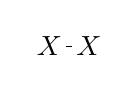
\begin{tikzpicture}[baseline={([yshift=-.5ex]current bounding box.center)}]
	\path (0,0) node (A) {$X$} ++ (0.5,0) node (B) {$X$};
	\draw (A) -- (B);
\end{tikzpicture}
\end{align}

We choose a particular 1-element set $\{*\}$ that acts as the identity in the sense that $\{*\}\times A\cong A\times \{*\} \cong A$ for any set $A$. The erase map $\text{del}_X:X\kto \{*\}$ defined by $(\text{del}_X)(*|x) = 1$ is a Markov kernel that ``discards the input''. It is drawn as a fuse:

\begin{align}
	\text{del}_X&:=\begin{tikzpicture}[baseline={([yshift=-.5ex]current bounding box.center)}]
	\path (0,0) ++ (1,0) node (B) {$X$};
	\draw[-{Rays[n=8]}] (A) -- (B);
\end{tikzpicture}
\end{align}

The copy map $\text{copy}_X:X\kto X\times X$ defined by $(\text{copy}_X)(x',x''|x)=\llbracket x=x' \rrbracket \llbracket x=x'' \rrbracket$ is a Markov kernel that makes two identical copies of the input. It is drawn as a fork:

\begin{align}
	\text{copy}_X&:=\begin{tikzpicture}[baseline={([yshift=-.5ex]current bounding box.center)}]
	\path (0,0) node (A) {$X$} 
	++ (0.5,0) node[copymap] (copy0) {}
	++ (0.5,0.15) node (B) {$X$}
	+ (0,-0.3) node (C) {$X$};
	\draw (A) -- (copy0) to [out=45,in=180] (B) (copy0) to [out=-45, in=180] (C);
\end{tikzpicture}
\end{align}

The swap map $\text{swap}_{X,Y}:X\times Y\kto Y\times X$ defined by $(\text{swap}_{X,Y})(y',x'|x,y)=\llbracket x=x' \rrbracket\llbracket y=y' \rrbracket$ swaps two inputs, and is represented by crossing wires:

\begin{align}
	\text{swap}_X &:=  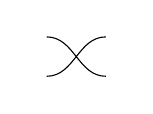
\begin{tikzpicture}[baseline={([yshift=-.5ex]current bounding box.center)}]
		\path (0,0) node (A) {} 
		+ (0,-0.5) node (B) {}
		++ (1,0) node (C) {}
		+ (0,-0.5) node (D) {};
		\draw (A) to [out=0,in=180] (D) (B) to [out=0, in=180] (C);
	\end{tikzpicture}
\end{align}

Because we anticipate that the graphical notation will be unfamiliar, we will include some examples in the next section.

\subsubsection{Examples}

When translating string diagram notation to integral notation, a number of identities can speed up the process.

For arbitrary $\kernel{K}:X\times Y\to Z$, $\kernel{L}:W\to Y$

\begin{align}
 [(\text{id}_X\otimes \kernel{L})\kernel{K}](A|x,w) &= \int_{Y}\int_X   \kernel{K}(z|x',y')\kernel{L}(dy'|w)\text{id}_X(dx'|x)\\
										   &= \int_Y  \kernel{K}(z|x,y') \kernel{L}(dy'|w)
\end{align}

That is, an identity map passes its input to the next kernel in the product. 

For arbitrary $\kernel{K}: X\times Y\times Y\to Z$ (where we apply the above shorthand in the first line):

\begin{align}
 [(\text{id}_X\otimes \text{copy}_Y)\kernel{K}](A|x,y) &= \int_Y\int_Y \kernel{K}(A|x,y',y'') \text{copy}_Y(dy'\times dy''|y)\\
										   &= \kernel{K}(A|x,y,y)
\end{align}

That is, the copy map passes along two copies of its input to the next kernel in the product. 

For a collection of kernels $\kernel{K}^n:Y^n\to Z$, $n\in[n]$, define $(y)^{n}=(y|i\in[n])$ and:

\begin{align}
	\text{copy}^n_Y &:= \begin{cases}
	\text{copy}^{n-1}_Y(\text{id}_{Y^{n-2}}\otimes \text{copy}_Y) & n>2\\
	\text{copy}_Y & n=2
	\end{cases}\\
	(\text{copy}^2_Y\kernel{K}^2)(z|y) &= \kernel{K}^2(z|y,y)\\
\end{align}

Suppose for induction
\begin{align}
(\text{copy}^{n-1}_Y\kernel{K}^{n-1})(z|y) &= \kernel{K}^{n-1}(z|(y)^{n-1})
\end{align}

then
\begin{align}
(\text{copy}^n_Y\kernel{K}^n)(z|y) &= (\text{copy}^{n-1}_Y(\text{id}_{Y^{n-2}}\otimes \text{copy}_Y)\kernel{K}^n)(z|y)\\
									 &= \sum_{y'\in Y^{n-1}}(\text{id}_{Y^{n-2}}\otimes \text{copy}_Y)(\mathbf{y}'|(y)^{n-1})\kernel{K}^n(z|\mathbf{y}')\\
									 &= \kernel{K}^n(z|(y)^n)
\end{align}

That is, we can define the $n$-fold copy map that passes along $n$ copies of its input to the next kernel in the product.

\subsubsection{Example: comb insertion}

The following examples illustrate 2-combs and the insertion operation, both of which we will define later. As an example in translating diagrams, we show how the diagrams for a 2-comb and 2-comb with an inserted Markov kernel can be translated to integral notation.

Consider the Markov kernels $\kernel{K}:W\kto X$, $\kernel{L}:X\times W\times Y\kto Z$ and the 2-comb $\kernel{M}:W\times Y\kto X\times Z$ defined as

\begin{align}
	\kernel{M} = \tikzfig{2_comb}\label{eq:2comb_M}
\end{align}

Following the rules above, we can translate this to ordinary notation by first breaking it down into products and tensor products, and then evaluating these products

\begin{align}
	\kernel{M}(A\times B|w,y) = [&(\text{copy}_W\otimes \text{id}_Y)(\kernel{K}\otimes \text{id}_{W\times Y})\\
	&(\text{copy}_X\otimes \text{id}_{W\times Y})(\text{id}_X\otimes\kernel{L})](A\times B|w,y)\\
						= [&(\kernel{K}\otimes \text{id}_{W\times Y})(\text{copy}_X\otimes \text{id}_{W\times Y})\\
						&(\text{id}_X\otimes\kernel{L})](A\times B|w,w,y)\\
						= \;&\int_{X}  (\text{id}_X\otimes\kernel{L})(A\times B|x',w,y) \kernel{K} (dx'|w)
						](y,z|y',x)\\
						= \;&\int_X \text{id}_X(A|x') \kernel{L}(B|x',w,y)\kernel{K}(dx'|w)\\
						= \;&\int_A \kernel{L}(B|x',w,y)\kernel{K}(dx'|w)
\end{align}

If we are given additionally $\kernel{J}:X\times W\kto Y$, we can define a new Markov kernel $\kernel{N}:W\kto Z$ given by ``inserting'' $\kernel{J}$ into $\kernel{M}$:

\begin{align}
	\kernel{N} = \tikzfig{2comb_inserted_anon}\label{eq:2comb_winsert}
\end{align}


We can translate Equation \ref{eq:2comb_winsert} to

\begin{align}
	\kernel{N}(A\times B\times C|w) = &[\text{copy}_W(\kernel{K}\text{copy}^3_Y\otimes \text{id}_W)\\
	&(\text{id}_Y\otimes\kernel{J}\otimes \text{id}_Y)(\text{id}_Y \otimes \text{copy}_X\otimes \text{id}_Y)\\
	&(\kernel{L}\otimes \text{id}_X\otimes \text{id}_Y)] (A\times B\times C|w)\\
					= &[(\kernel{K}\text{copy}^3_Y\otimes \text{id}_W)(\text{id}_Y\otimes\kernel{J}\otimes \text{id}_Y)\\
					&(\text{id}_Y \otimes \text{copy}_X\otimes \text{id}_Y)\\
					&(\kernel{L}\otimes \text{id}_X\otimes \text{id}_Y)] (A\times B\times C|w,w)\\
					= &\int_X\int_Y\kernel{L}(C|x',w,y') \text{id}_X(A|x') \text{id}_Y(B|y') \kernel{J}(dy'|x',w)\kernel{K}(dx'|w)\\
					= &\int_A\int_B\kernel{L}(C|x',w,y') \kernel{J}(dy'|x',w)\kernel{K}(dx'|w)
\end{align}
\subsection{Semantics of observed and unobserved variables}\label{sec:variables}

We are interested in constructing \emph{probabilistic models} which explain some part of the world. In a model, variables play the role of ``pointing to the parts of the world the model is explaining''. Both observed an unobserved variables play important roles in causal modelling and we think it is worth clarifying what variables of either type refer to. Our approach is a standard one: a probabilistic model is associated with an experiment or measurement procedure that yields values in a well-defined set. Observable variables are obtained by applying well-defined functions to the result of this total measurement. We use a richer sample space that includes ``unobserved variables'' that are formally treated the same way as observed variables, but aren't associated with any real-world counterparts.

Consider Newton's second law in the form $\proc{F}=\proc{MA}$ as a simple example of a model that relates variables $\proc{F}$, $\proc{M}$ and $\proc{A}$. As \citet{feynman_feynman_1979} noted, this law is incomplete -- in order to understand it, we must bring some pre-existing understanding of force, mass and acceleration as independent things. Furthermore, the nature of this knowledge is somewhat perculiar. Acknowledging that physicists happen to know a great deal about forces on an object, it remains true that in order to actually say what the net force on a real object is, even a highly knowledgeable physicist will still have to go and do some measurements, and the result of such measurements will be a vector representing the net forces on that object.

This suggests that we can think about ``force'' $\proc{F}$ (or mass or acceleration) as a kind of procedure that we apply to a particular real world object and which returns a mathematical object (in this case, a vector). We will call $\proc{F}$ a \emph{procedure}. Our view of $\proc{F}$ is akin to \citet{menger_random_2003}'s notion of variables as ``consistent classes of quantities'' that consist of pairing between real-world objects and quantities of some type. Force $\proc{F}$ itself is not a well-defined mathematical thing, as measurement procedures are not mathematically well-defined. At the same time, the set of values it may yield \emph{are} well-defined mathematical things.

We will assume that any procedure will eventually yield an unambiguous value in a defined mathematical set. No actual procedure can be guaranteed to have this property -- any apparatus, however robust, could suffer catastrophic failure -- but we assume that we can study procedures reliable enough that we don't lose much by making this assumption. This assumption allows us to say a procedure $\proc{B}$ yields values in $B$. $\proc{B}\yields x$ is the proposition that $\proc{B}$, when completed, yields the value $x\in B$, and by assumption exactly one of these propositions is true. For $A\subset B$, $\proc{B}\yields A$ is the proposition $\lor_{x\in A} \proc{B}\yields x$. Two procedures $\proc{B}$ and $\proc{C}$ are the same if $\proc{B}\yields x\iff \proc{C}\yields x$ for all $x\in B$. 

The notion of ``yielding values'' allows us to define an operation akin to function composition. If I have a procedure $\proc{B}$ that takes values in some set $B$, and a function $f:B\to C$, define the ``composition'' $f\circ \proc{B}$ to be the procedure $\proc{C}$ that yields $f(x)$ whenever $\proc{B}$ yields $x$. For example, $\proc{MA}$ is the composition of $h:(x,y)\mapsto xy$ with the procedure $(\proc{M},\proc{A})$ that yields the mass and acceleration of the same object. Composition is associative - for all $x\in B$: 

\begin{align}
	(g\circ f)\circ\proc{B}\text{ yields } x &\iff B\text{ yields } (g\circ f)^{-1}(x) \\
	&\iff B\text{ yields } f^{-1}(g^{-1}(x))\\
	&\iff f\circ B \text{ yields } g^{-1}(x)\\
	&\iff g\circ(f\circ B)\text{ yields } x
\end{align}


One might whether there is also some kind of ``append'' operation that takes a standalone $\proc{M}$ and a standalone $\proc{A}$ and returns a procedure $(\proc{M},\proc{A})$. Unlike function composition, this would be an operation that acts on two procedures rather than a procedure and a function. Rather than attempt to define any operation of this type, we simply assume that somehow a procedure has been devised that measures everything of interest, which we will call $\proc{S}$ which takes values in $\Psi$. We assume $\proc{S}$ is such that any procedure of interest can be written as $f\circ \proc{S}$ for some $f$.

For the model $\proc{F}=\proc{MA}$, for example, we could assume $\proc{F}=f\circ \proc{S}$ for some $f$ and $(\proc{M},\proc{A})=g\circ \proc{S}$ for some $g$. In this case, we can get $\proc{MA}=h\circ(\proc{M},\proc{A})=(h\circ g)\circ\proc{S}$. Note that each procedure is associated with a unique function with domain $\Psi$.

Thus far, $\Psi$ is a ``sample space'' that only contains observable variables. To include unobserved variables, we posit a richer sample space $\Omega$ such that the measurement $\proc{S}$ determines an element of some partition of $\Omega$ rather than an element of $\Omega$ itself. Then, by analogy to procedures defined with respect to $\proc{S}$, we identify variables in general with measurable functions defined on the domain $\Omega$. 

Specifically, suppose $\proc{S}$ takes values in $\Psi$. Then we can propose a sample space $\Omega$ such that $|\Omega|\geq |\Psi|$ and a surjective function $\RV{S}:\Omega\to \Psi$ associated with $\proc{S}$. We connect $\Omega$, $\RV{S}$ and $\proc{S}$ with the notion of \emph{consistency with obseravation}:

\begin{align}
 &\omega\in \Omega\text{ is \emph{consistent with observation} iff the result yielded by }\proc{S}\text{ is equal to }\RV{S}(\omega)\label{def:observable}
\end{align}

Thus the procedure $\proc{S}$ eventually restricts the observationally consistent elements of $\Omega$. If $\proc{S}$ yield the result $s$, then the consistent values of $\Omega$ will be $\RV{S}^{-1}(s)$.

One thing to note in this setup is that two different sets of measurement outcomes $\Psi$ and $\Psi'$ entail a different mesurement procedures $\proc{S}$ and $\proc{S}'$, but different sample spaces $\Omega$ and $\Omega'$ may be used to model a single procedure $\proc{S}$. We will sometimes consider different models of the same observable procedures.

As far as we know, distinguishing variables from procedures is somewhat nonstandard, but it is a useful distinction to make. While they may not be explicitly distinguished, both variables and procedures are often discussed in statistical texts. For example, \citet{pearl_causality:_2009} offers the following two, purportedly equivalent, definitions of variables:
\begin{quote}
By a \emph{variable} we will mean an attribute, measurement or inquiry that may take on one of several possible outcomes, or values, from a specified domain. If we have beliefs (i.e., probabilities) attached to the possible values that a variable may attain, we will call that variable a random variable.
\end{quote}

\begin{quote}
This is a minor generalization of the textbook definition, according to which a random variable is a mapping from the sample space (e.g., the set of elementary events) to the real line. In our definition, the mapping is from the sample space to any set of objects called ``values,'' which may or may not be ordered.
\end{quote}

Our view is that the first definition is a definition of a procedure, while the second is a definition of a variable. Variables model procedures, but they are not the same thing. We can establish this by noting that, under our definition, every procedure of interest -- that is, all procedures that can be written $f\circ \proc{S}$ for some $f$ -- is modeled by a variable, but there may be variables defined on $\Omega$ that do not factorise through $\proc{S}$, and these variables do not model procedures.

\subsection{Events}

To recap, we have a procedure $\proc{S}$ yielding values in $\Psi$ that measures everything we are interested in, a sample space $\Omega$ and a function $\RV{S}$ that models $\proc{S}$ in the sense of Definition \ref{def:observable}. We assume also that $\Psi$ has a $\sigma$-algebra $\sigalg{E}$ (this may be the power set of $\Psi$, as measurement procedures are typically limited to finite precision). $\Omega$ is equipped with a $\sigma$-algebra $\sigalg{F}$ such that $\sigma(\RV{S})\subset \sigalg{F}$. If a procedure $\proc{X}=f\circ \RV{S}$ then we define $\RV{X}:\Omega\to X$ by $\RV{X}:=f\circ\RV{S}$.

If a particular procedure $\proc{X}=f\circ \proc{S}$ eventually yields a value $x$, then the values of $\Omega$ consistent with observation must be a subset of $\RV{X}^{-1}(x)$. We define an \emph{event} $\RV{X}\yields x:\equiv \RV{X}^{-1}(x)$, which we read ``the event that $\RV{X}$ yields x''. An event $\RV{X}\yields x$ occurs if the consistent values of $\Omega$ are a subset of $\RV{X}\yields x$, thus ``the event that $\RV{X}$ yields x occurs$\equiv \proc{X}$ yields $x$''. The definition of events applies to all types of variables, not just observables, but we only provide an interpretation of events ``occurring'' when the variable $\RV{X}$ is associated with some $\proc{X}$.

For measurable $A\in \sigalg{X}$, $\RV{X}\yields A=\bigcup_{x\in A} \RV{X}\yields x$. 

Given $\RV{Y}:\Omega\to X$, we can define a sequence of variables: $(\RV{X},\RV{Y}):=\omega\mapsto (\RV{X}(\omega),\RV{Y}(\omega))$. $(\RV{X},\RV{Y})$ has the property that $(\RV{X},\RV{Y})\yields (x,y)= \RV{X}\yields x\cap \RV{Y}\yields y$, which supports the interpretation of $(\RV{X},\RV{Y})$ as the values yielded by $\RV{X}$ and $\RV{Y}$ together.

It is common to use the symbol $=$ instead of $\bowtie$, but we want to avoid this because $\RV{Y}=y$ already has a meaning, namely that $\RV{Y}$ is a constant function everywhere equal to $y$. 

\subsection{Probabilistic models for causal inference}

The sample space $(\Omega,\sigalg{F})$ along with our collection of variables is a ``model skeleton'' -- it tells us what kind of data we might see. The process $\proc{S}$ which tells us which part of the world we're interested in is related to the model $\Omega$ and the observable variables by the criterion of \emph{consistency with observation}. The kind of problem we are mainly interested in here is one where we make use of data to help make decisions under uncertainty. Probabilistic models have a long history of being used for this purpose, and our interest here is in constructing probabilistic models that can be attached to our variable ``skeleton''. 

For causal inference, we find we need to generalise the standard approach to constructing probability models on a given sample space $(\Omega,\sigalg{F})$. The key things we need to handle are \emph{gaps} in our model. \citet{hajek_what_2003} defines \emph{probability gaps} as propositions that do not have a probability assigned to them. Our view of probability gaps is slightly different -- in this work, a model with probability gaps as one that is missing some key parts. If we complete such a model with parts of the appropriate type, we get a standard probability model.

Probability gaps are useful in models used for decision making because, when I have a number of different options I could choose, a model can only help select from them if it tells me what is likely to happen for each choice I could make. Thus if we have a variable representing choices, we must have a model that can tolerate a probability gap for this variable.

As an initial example of a probability gap in causal inference, we will consider the example of truncated factorisation. For this example, we will assume that the reader is familiar enough with marginal probabilities, conditional probabilities and causal models to follow along. We will offer more careful definitions of terms later.

Suppose we have a causal Bayesian network $(\prob{P}^{\RV{XYZ}},\mathcal{G})$ where $\RV{X}:\Omega\to X$, $\RV{Y}:\Omega\to Y$ and $\RV{Z}:\Omega\to Z$ are variables, $\prob{P}^{\RV{XYZ}}$ is a probability measure on $X\times Y\times Z$ that we call ``a probability model of $(\RV{X},\RV{Y},\RV{Z})$'' and $\mathcal{G}$ is a Directed Acyclic Graph whose vertices we identify with $\RV{X}$, $\RV{Y}$ and $\RV{Z}$ that contains the edges $\RV{X}\longrightarrowRHD \RV{Y}$ and $\RV{X}\longleftarrowRHD \RV{Z} \longrightarrowRHD \RV{Y}$. ``Setting $\RV{X}$ to $x$'' is an operation that takes as inputs $\prob{P}^{\RV{XYZ}}$, $\mathcal{G}$ and some $x\in X$ and returns a new probability measure $\prob{P}_x^{\RV{XYZ}}$ on $X\times Y\times Z$ given by \citep[page ~24]{pearl_causality:_2009}:
\begin{align}
	\prob{P}^{\RV{XYZ}}_{x}(x',y,z)=\disint{P}^{\RV{Y|XZ}}(y|x,z)\prob{P}^{\RV{Z}}(z)\llbracket x=x' \rrbracket\label{eq:truncated_fac}
\end{align}

Equation \ref{eq:truncated_fac} embodies three assumptions about a model of the operation of ``setting $\RV{X}$ to $x$''. First, such a model must assign probability 1 to the proposition that $\RV{X}$ yields $x$. Second, such a model must assign the same marginal probability distribution to $\RV{Z}$ as the input distribution; $\prob{P}^{\RV{Z}}=\prob{P}_{x}^{\RV{Z}}$. Finally, our model must also assign the same conditional probability to $\RV{Y}$ given $\RV{X}$ and $\RV{Z}$; $\prob{P}^{\RV{Y}|\RV{XZ}}=\prob{P}_x^{\RV{Y}|\RV{XZ}}$.

Notice that the map $x\mapsto \prob{P}^{\RV{XYZ}}_x$ itself ``looks like'' a conditional probability. It maps each $x\in X$ to a probability distribution over $(\RV{X},\RV{Y},\RV{Z})$. In fact, a popular alternative notation for $\prob{P}^{\RV{XYZ}}_x$ this map is $\prob{P}^{\RV{XYZ}|do(\RV{X}=x)}$, which is clearly suggestive of an interpretation as a kind of conditional probability. We will take this interpretation seriously: we will posit some variable $\RV{U}$ (which may or may not be observable) and a probabilisitic model $\prob{Q}^{\RV{XYZ}|\RV{U}}:=x\mapsto \prob{P}^{\RV{XYZ}}_x$.

We note that the thing called $do(\RV{X}=x)$ or that we have called $\RV{U}$ is often referred to as an \emph{intervention}. Interventions are often things we can choose to do or not to do. Also, perhaps, we could also consider choosing to do or not do an intervention based on the output of some random process. In this case, we will need a model that can tell us which result we are likely to see for any choice of $\prob{Q}_\alpha^{\RV{U}}$; the distribution of $\RV{U}$ is a \emph{probability gap}.

$\prob{Q}^{\RV{XYZ}|\RV{U}}$, as we have defined it so far, is not quite an ideal candidate for for a gappy probability model. Firstly, because conditional probabilities are arbitrary on sets of measure zero with regard to $\prob{P}^{\RV{XYZ}}$, definition \ref{eq:truncated_fac} can be satisfied by multiple probability distributions that differ in meaningful ways. Suppose $\RV{X}$, $\RV{Y}$ and $\RV{Z}$ are binary, $\prob{P}^{\RV{Z}}(1)=1$ and $\prob{P}(\RV{X}\yields \RV{Z})=1$. Then we can consistently choose $\prob{P}^{\RV{Y|XZ}}(1|0,1)=1$ or $\prob{P}^{\RV{Y|XZ}}(1|0,1)=0$ because $\{0,1\}$ is a measure zero event. However, the first choice gives us  $\prob{P}^{\RV{XYZ}}_{0}(0,1,1)=1$ while the second gives us $\prob{P}^{\RV{XYZ}}_{0}(0,1,1)=0$, which are very different opinions regarding ``the result of setting $\RV{X}$ to $1$''.

Secondly, there may be no probability model at all that satisfies Equation \ref{eq:truncated_fac}. For example, suppose $\RV{X}=f\circ\RV{Z}$ for some $f$. Then we must have $\prob{P}^{\RV{X}}_x(x')=\prob{P}^{\RV{Z}}_x(f^{-1}(x'))$ for any $x$. However, we also have $\prob{P}^{\RV{X}}_x(x')=\llbracket x = x' \rrbracket$ for all $x,x'$ and $\prob{P}^{\RV{Z}}_x=\prob{P}^{\RV{Z}}$ for all $x$. Thus if $\RV{X}$ can more than one value, there is at least one choice of $x$ that cannot simultaneously satisfy these requirements.

This might seem like an absurd model, but an analogous causal graph appears in \citet{shahar_association_2009} where $\RV{Z}=(\RV{H},\RV{W})$, representing a person's height and weight, and $\RV{X}$ represents their body mass index, which is to say $\RV{X}=\frac{\RV{W}}{\RV{H}^2}$. Furthermore, this paper uses this model to argue that body mass index cannot have a causal effect. Such an argument cannot be supported by Equation \ref{eq:truncated_fac} because by that equation there is no probability model corresponding to an intervention on $\RV{X}$.

Our first aim is to offer a more careful theory of probability models with gaps in them, addressing these two shortcomings.

\subsection{Probability gaps}

Probability gap models are probability models that are missing key parts. If we provide a ``missing part'' or ``insert'' of the right type then we get a probability model. That is, a probability gap model is in general a function from something to a probability model. We consider specific kinds of probability gap models that take marginal probabilities or conditional probabilities to probability models.

\begin{definition}[Probability gap model]
Given a fundamental probability set $\Omega$ and a set of inserts $A$, a probability gap model $\prob{P}:A\to \Delta(\Omega)$ is a function that sends an element of $A$ to a probability measure on $\Omega$, which we call a \emph{base measure}.
\end{definition}

We will make a substantial simplifying assumption: all sets, including the sample space $\Omega$ and any set of values a variable takes, are discrete sets. That is, they are at most countably infinite and the $\sigma$-algebra of measurable sets is the power set. Because we are working with discrete sets we will by convention call probability measures on set elements: $\prob{P}^{\RV{X}}(x):=\prob{P}^{\RV{X}}(\{x\})$. 

\begin{definition}[Probability space]
A probability space is a triple $(\mu,\Omega,\sigalg{F})$, where $\mu$ is a probability measure on $\sigalg{F}$ which we here take to be $\mathscr{P}(\Omega)$. We call $\mu$ the \emph{base measure}.
\end{definition}

Probability spaces along with random variables can be used to define probability distributions of those random variables. We call such distributions \emph{pushforwards}.

\begin{definition}[Pushforward]\label{def:pushforward}
Given a probability space $(\mu,\Omega)$ and a random variable $\RV{X}:\Omega\to X$, we can define the probability distribution $\mu^{\RV{X}}:\sigalg{X}\to [0,1]$ of $\RV{X}$ as the \emph{pushforward} of $\mu$ by $\RV{X}$. Specifically, for any $x\in X$, $\mu^{\RV{X}}(x):=\mu(\RV{X}\yields x)$. 
\end{definition}

A $\RV{Y}|\RV{X}$-\emph{disintegration} is ``the probability of $\RV{Y}$ given $\RV{X}$ relative to $\mu$''. It is a Markov kernel that maps a pushforward of $\RV{X}$ to the pushforward of the sequence $(\RV{X},\RV{Y})$.

\begin{definition}[Disintegration]\label{def:disint}
Given a probability space $(\mu,\Omega)$ and random variables $\RV{X}:\Omega\to X$, $\RV{Y}:\Omega\to Y$, the disintegration $\overline{\mu}^{\RV{Y}|\RV{X}}:X\kto Y$ is any Markov kernel such that
\begin{align}
	\mu^{\RV{X}}(x)\overline{\mu}^{\RV{Y}|\RV{X}}(y|x)&= \mu^{\RV{XY}}(x,y) &\forall x\in X, y\in Y\\
	&\iff\\
	\tikzfig{disint_def} &= \mu^{\RV{XY}}
\end{align}
Because in general disintegrations are non-unique and we sometimes need to account for this fact, we use a bar over the top of the letter to indicate that it is an arbitrary element of the set of disintegrations.
\end{definition}

Given a probability gap model $\prob{P}$, we define pushforwards and disintegrations as probability measures and Markov kernels that satisfy Definitions \ref{def:pushforward} and \ref{def:disint} respectively for all base measures in the range of $\prob{P}$.

\begin{definition}[Pushforward - probability gap model]
Given a fundamental probability set $\Omega$, a set of inserts $A$, a variable $\RV{X}:\Omega\to X$ and a probability gap model $\prob{P}:A\to \Delta(\Omega)$, if $\prob{P}_a^{\RV{X}}=\prob{P}_{a'}^{\RV{X}}$ for all $a,a'\in A$, the pushforward $\prob{P}^{\RV{X}}=\prob{P}_a\right)^{\RV{X}}$ for any $a$. Otherwise, it is undefined.
\end{definition}

\begin{definition}[Disintegration - probability gap model]
Given a fundamental probability set $\Omega$, a set of inserts $A$, variables $\RV{X}:\Omega\to X$ and $\RV{Y}:\Omega\to Y$ and a probability gap model $\prob{P}:A\to \Delta(\Omega)$, $\disint{P}^{\RV{Y}|\RV{X}}$ is any Markov kernel $X\kto Y$ such that for all $\prob{P}_a:=\prob{P}(a)$, $a\in A$
\begin{align}
	\prob{P}_a^{\RV{X}}(x)\disint{P}^{\RV{Y}|\RV{X}}(y|x)&= \prob{P}_a^{\RV{XY}}(x,y) &\forall x\in X, y\in Y
\end{align}
If no such Markov kernel exists, $\disint{P}^{\RV{Y}|\RV{X}}$ is undefined.
\end{definition}

Given a disintegration of a probability gap model, we can find other disintegrations by pushing forward.

\begin{theorem}[Recursive pushforward]\label{th:recurs_pushf}
Suppose we have a fundamental probability set $\Omega$, a set of inserts $A$, variables $\RV{X}:\Omega\to X$ and $\RV{Y}:\Omega\to Y$, $\RV{Z}:\Omega\to Z$ and a probability gap model $\prob{P}:A\to \Delta(\Omega)$ such that $\disint{P}^{\RV{X}|\RV{Y}}$ is a $\RV{Y}|\RV{X}$ disintegration of $\prob{P}$ and $\RV{Z}=f\circ \RV{Y}$ for some $f:Y\to Z$. Then there exists a pushforward $\prob{P}^{\RV{Z}|\RV{Z}}$ defined by $\prob{P}^{\RV{Z}|\RV{Z}}(z|x):=\prob{P}^{\RV{Y}|\RV{X}}(f^{-1}(z)|x)$.
\end{theorem}

\begin{proof}
For any $a\in A$, $x,z$
\begin{align}
\prob{P}_a^{\RV{X}}(x)\prob{P}_a^{\RV{Z}|\RV{X}}(z|x) &= \prob{P}_a(\RV{X}^{-1}(x)\cap\RV{Z}^{-1}(z))\\
					   &= \prob{P}_a(\RV{X}^{-1}(x)\cap\RV{Y}^{-1}(f^{-1}(z)))\\
					   &= \prob{P}_a^{\RV{X},\RV{Y}}(\{x\}\times f^{-1}(z))\\
					   &= \prob{P}_a^{\RV{X}}(x)\prob{P}_a^{\RV{Y}|\RV{X}}(f^{-1}(z)|x)
\end{align}
\end{proof}

\subsection{Probability gap models defined by disintegrations and pushforwards}

In the previous section we saw how we can define disintegrations and pushforwards of probability gap models. Here, we will see how to define probability gap models by specifying a collection of disintegratons and pushforwards. In fact, we will define a hierarchy of gap models -- a model specified by a probability distribution is an order zero gap model while a model specified by a conditional probability is an order 1 gap model. An order $n$ gap model maps its inserts to order $n-1$ gap models. 

To develop this idea, it will be helpful to define an operation $\odot$ that combines Markov kernels in the manner of Definition \ref{def:disint}.

\begin{definition}[Copy-product]\label{def:copyproduct}
Given two Markov kernels $\prob{K}:X\kto Y$ and $\prob{L}:Y\times X\kto Z$, define the copy-product $\prob{K}\odot\prob{L}:X\to Y\times Z$ as
\begin{align}
	\prob{K}\odot\prob{L}:&= \text{copy}_X(\prob{K}\otimes \text{id}_X)(\text{copy}_Y\otimes\text{id}_X )(\text{id}_Y \otimes \prob{L})\\
							&= \tikzfig{copy_product}\\
							&\iff\\
	(\prob{K}\odot\prob{L})(y,z|x) &= \prob{L}(z|y,x)\prob{K}(y|x)
\end{align}
\end{definition}

Given a variable $\RV{X}:\Omega\to X$ and an arbitrary probability measure on $X$ which we will call $\prob{P}^{\RV{X}}$, we want $\prob{P}:A\to \Delta(\Omega)$ to be some probability gap model such that $\prob{P}^{\RV{X}}$ is a pushforward of $\prob{P}$. Note that for any $a\in A$, defining $\RV{I}:\Omega\to \Omega$ to be the variable given by the identity function on $\Omega$, by the existence of disintegrations (Lemma \ref{lem:disint_exist}) there exists some $\disint{P}_a^{\RV{I}|\RV{X}}$ such that $\prob{P}_a^{\RV{X}\RV{I}}=\prob{P}^{\RV{X}}\odot \prob{P}^{\RV{I}|\RV{X}}$. 

Alternatively, we could \emph{define} $\prob{P}$ to be a function from Markov kernels $X\kto \Omega$ to probability distributions on $\Omega$ such that for some $\kernel{K}:X\kto \Omega$, $\prob{P}(\kernel{K})=\prob{P}^{\RV{X}}\odot \prob{K}$. However, $\prob{P}$ cannot in general be defined for \emph{every} Markov kernel $X\kto \Omega$, as for many such kernels the product $\prob{P}^{\RV{X}}\odot \prob{K}$ will not be the pushforward of any base measure on $\Omega$. For example, let $X=\Omega=\{0,1\}$ and $\RV{X}=\RV{I}$ and $\kernel{K}(\omega|x) = \llbracket 1 - x \rrbracket$. Then if we suppose $\prob{P}^{\RV{X}}\odot \prob{K}=\prob{P}_{\prob{K}}^{\RV{XX}}$, we find that $\prob{P}_{\prob{K}}^{\RV{XX}}(x,x)=\prob{P}_{\prob{K}}(\RV{X}\yields x)=0$ for all $x\in X$, so this is not possible.

It is also sometimes possible to find probability measures $\prob{P}^{\RV{X}}$ on $\Delta(X)$ such that no base measure on $\Omega$ pushes forward via $\RV{X}$ to $\prob{P}^{\RV{X}}$. Consider, for example, $\RV{X}=(\RV{Y},\RV{Y})$ for some $\RV{Y}$ and any measure that assigns nonzero probability to $(\RV{Y},\RV{Y})\yields (y,y')$ for $y\neq y'$.

We can, however, define a probability gap model $\prob{P}$ induced by some \emph{valid probability distribution} $\prob{P}^{\RV{X}}\in \Delta(X)$ to be the map from all \emph{valid completions} $X\kto \Omega$ to probability measues on $\Omega$. 

\begin{definition}[Valid probability distribution]\label{def:valid_dist}
A valid $\RV{X}$ probability distribution $\prob{P}^{\RV{X}}$ is any probability mesure on $\Delta(X)$ such that $\RV{X}^{-1}(x)=\emptyset\implies \prob{P}^{\RV{X}}(x) = 0$.
\end{definition}

\begin{definition}[Valid conditional probability]\label{def:valid_conditional_prob}
Given $(\Omega,\sigalg{F})$, $\RV{X}:\Omega\to X$, $\RV{Y}:\Omega\to Y$ a \emph{valid $\RV{Y}|\RV{X}$ conditional probability} $\prob{P}^{\RV{Y}|\RV{X}}$ is a Markov kernel $X\kto Y$ such that it assigns probability 0 to contradictions:
\begin{align}
	\forall y\in Y, x\in X: (\RV{X},\RV{Y})\yields(x,y) = \emptyset \implies \left(\prob{P}^{\RV{Y}|\RV{X}}(y|x) = 0\right) \lor \left(\RV{X}\yields (x) = \emptyset\right)
\end{align}
\end{definition}

The typical definition of conditional probability allows for conditional probabilities that are invalid by this definition. See Theorem \ref{th:valid_disint} for a proof that it is at least always possible to choose a valid conditional probability from among the options available under the usual definition. See also \citet{hajek_what_2003} for arguments in favour of requiring conditional distributions satisfy something like Definition \ref{def:valid_conditional_prob}.

\begin{definition}[Order 0 probability gap model]
An order 0 probability gap model $\prob{P}$ is defined by a variable $\RV{X}:\Omega\to X$ and a valid probability distribution $\prob{P}^{\RV{X}}$, and is the map from valid conditional probabilities $X\kto \Omega$ to base measures given by
\begin{align}
	\prob{P}_{\kernel{K}} = \prob{P}^{\RV{X}}\odot\kernel{K}$
\end{align}
for any valid conditional probability $\kernel{K}$.
\end{definition}

Theorem \ref{th:completion} shows that these definitions are sufficient to ensure that $\prob{P}$ is a well-defined probability gap model that has the pushforward $\prob{P}^{\RV{X}}$, and the validity of $\model{J}$ is necessary.

\begin{theorem}[Completion]\label{th:completion}
Given $\RV{X}:\Omega\to X$, $\kernel{J}\in \Delta(X)$ and $\kernel{K}:X\kto \Omega$, there exists some $\mu$ $\RV{Y}:\Omega\to Y$ such that $\kernel{J}\odot \kernel{K}=\mu^{\RV{Y}}$ and $\mu^{\RV{X}}=\kernel{J}$ if $\kernel{J}$ is a valid probability distribution and $\kernel{K}$ is a valid conditional probability, and only if $\kernel{J}$ is a valid probability distribution.
\end{theorem}

\begin{proof}
If:
Define $\mu$ by
\begin{align}
	\mu(\omega) &= \sum_{x\in X} (\kernel{J}\odot \kernel{K})(x,\omega)
\end{align}
Then
\begin{align}
	\mu^{\RV{X}}(x) &= \mu (\RV{X}\yields x)\\
	&= \sum_{x'\in X} \kernel{J}(x') \kernel{K}(\RV{X}\yields x|x')\\
	&= \sum_{x'\in X} \kernel{J}(x') \llbracket x=x'\rrbracket&\text{if }\RV{X}\yields x \neq \emptyset\\
	&= \kernel{J}(x)
\end{align}
and, letting $\RV{Y}=(\RV{X},\RV{I})$, for any $x\in X$, $\omega\in \Omega$
\begin{align}
	\mu^{\RV{Y}}(x,\omega) &= \mu^{\RV{XI}}(x,\omega)\\
	&= \mu(\omega)\overline{\mu}^{\RV{X}|\RV{I}}(x|\omega)\\
	&= \sum_{x'\in X} (\kernel{J}\odot \kernel{K})(x',\omega) \llbracket \RV{X}(\omega) = x \rrbracket\\
	&= (\kernel{J}\odot \kernel{K})(x,\omega)\\
	&\iff\\
	\kernel{J}\odot \kernel{K}&=\mu^{\RV{Y}}
\end{align}
Only if:
Suppose $\kernel{J}$ is not a valid probability distribution. Then there is some $x\in X$ such that $\RV{X}\yields x = \emptyset$ but $\kernel{J}(x)>0$. Then
\begin{align}
	\mu^{\RV{X}}(x) &= \mu (\RV{X}\yields x)\\
	&= \sum_{x'\in X} \kernel{J}(x') \kernel{K}(\RV{X}\yields x|x')\\
	&= 0\\
	&\neq \kernel{J}(x)
\end{align}
\end{proof}

\subsection{Higher order gap models}\label{sec:validity_of_gapprob}

Order 1 gap models are represented by \emph{conditional probabilities} and order 2 gap models by \emph{probability 2-combs}. We combine order 0 gap models (probability distributions) with order 1 gap models (conditional probabilities) using the ``copy-product'' $\odot$ to yield an order 0 gap model, and combine order 1 gap models with order 2 gap models usint the ``insert'' operation to yield order 1 gap models.

\textbf{A note on terminology:} We notate probability gap models with blackboard letters $\prob{P}$ and the Markov kernels that represent them with superscripts such as $\prob{P}^{\RV{Y}|\RV{X}}$. We use subscripts to indicate application of the model to an insert $\prob{P}_\alpha:=\prob{P}(\prob{P}^{\RV{X}}_\alpha)$, and $\prob{P}_\alpha$ is also a model of lower order. The same base letter with different superscripts $\prob{P}^{\RV{A}|\RV{B}}$ indicates a disintegration of $\prob{P}$, and $\RV{A}\CI_{\prob{P}} \RV{B}$ is a statement of independence with respect to the model $\prob{P}$.

\begin{definition}[Order 1 probability gap model]
An order 1 probability gap model $\prob{P}$ is defined by variables $\RV{X}:\Omega\to X$ and $\RV{Y}:\Omega\to Y$ and a valid conditional probability distribution $\disint{P}^{\RV{Y}|\RV{X}}$, and $\prob{P}$ is the map from valid $\RV{X}$ probability distributions to valid $(\RV{X},\RV{Y})$ probability distributions given by
\begin{align}
	\prob{P}_{\alpha}^{\RV{XY}} = \prob{P}_\alpha^{\RV{X}}\odot\prob{P}^{\RV{Y}|\RV{X}}
\end{align}
for any valid $\RV{X}$ probability distribution $\prob{P}_\alpha^{\RV{X}}$. The notation $\prob{P}^{\square \RV{Y}|\RV{X}}$ is shorthand for the model $\prob{P}$ defined by a conditional probability $\disint{P}^{\RV{Y}|\RV{X}}$ (it is useful to distinguish a model from a disintegration of a model).
\end{definition}

Note that the same model $\prob{P}$ may be represented by different $\disint{P}^{\RV{Y}|\RV{X}}$; this can happen wherever $\text{Range}(\RV{X})\neq X$ (for example, $\RV{X}=(\RV{Z},\RV{Z})$ for some $\RV{Z}$). 

We required order 0 probability gap models to be valid so that they extended to base measures in the appropriate way, and we similarly require a property of validity in order to ensure that an order 1 probability gap model $\prob{P}$ returns valid order 0 probability gap models $\prob{P}_\alpha$. Theorem \ref{th:valid_conditional_probability} shows that the property of validity (Definition \ref{def:valid_conditional_prob}) is necessary and sufficient for $\prob{P}$ to return valid order 0 probability gap models.

First, we show that Definitions \ref{def:valid_dist} and \ref{def:valid_conditional_prob} define equivalent notions of validity.

\begin{lemma}[Equivalence of validity definitions]\label{th:valid_agree}
Given $\RV{X}:\Omega\to X$, with $\Omega$ and $X$ discrete, a probability distribution $\prob{P}^{\RV{X}}$ is valid if and only if the conditional probability $\prob{P}^{\RV{X}|*}:=*\mapsto \prob{P}^{\RV{X}}$ is valid.
\end{lemma}

\begin{proof}
$*\yields *=\Omega$ necessarily. Thus validity of $\prob{P}^{\RV{X}|*}$ means 

\begin{align}
	\forall x\in X: \RV{X}\yields (x)=\emptyset \implies \prob{P}^{\RV{X}|*}(x|*)&=0\\
	&= \prob{P}^{\RV{X}}(x)\label{eq:nec_and_suff}
\end{align}

If: We refer to \citet{ershov_extension_1975} Theorem 2.5 for the proof that Equation \ref{eq:nec_and_suff} is necessary and sufficient for the existence of $\prob{P}^{\RV{I}}$ such that $\prob{P}^{\RV{I}}(\RV{X}^{-1}(A))=\prob{P}^{\RV{X}}(A)$ for all $A\in \sigalg{X}$ when $(\Omega,\sigalg{F})$ and $(X,\sigalg{X})$ are standard measurable. If $\Omega$ and $X$ are discrete, then they are standard measurable.

Only if: If $\RV{X}\yields x=\emptyset$ then $\prob{P}^{\RV{X}}(x)=\prob{P}^{\RV{I}}(\emptyset)=0$.
\end{proof}

Next, we show that 

\begin{theorem}[Product of valid conditional probabilities is valid]\label{lem:valid_extendability}
Given $(\Omega,\sigalg{F})$, $\RV{X}:\Omega\to X$, $\RV{Y}:\Omega\to Y$, $\RV{Z}:\Omega\to Z$ and any valid conditional probabilities $\prob{P}^{\RV{Y}|\RV{X}}$ and $\prob{Q}^{\RV{Z}|\RV{Y}\RV{X}}$, $ \prob{P}^{\RV{Y}|\RV{X}}\odot \prob{Q}^{\RV{Z}|\RV{Y}\RV{X}}$ is also a valid conditional probability.
\end{theorem}

\begin{proof}
Let $\prob{R}^{\RV{YZ}|\RV{X}}:=\prob{P}^{\RV{Y}|\RV{X}}\odot \prob{Q}^{\RV{Z}|\RV{Y}\RV{X}}$.

We only need to check validity in $x\in \RV{X}(\Omega)$, as it is automatically satisfied for other values of $\RV{X}$.

For all $x\in \RV{X}(\Omega)$, $\RV{X}\yields x\cap\RV{Y}\yields y=\emptyset$, $\prob{P}^{\RV{Y}|\RV{X}}(y|x)=0$ by validity. Thus
\begin{align}
	\prob{R}^{\RV{YZ}|\RV{X}}(y,z|x) &= \prob{Q}^{\RV{Z}|\RV{YX}}(z|y,x)\prob{P}^{\RV{Y}|\RV{X}}(y|x)\\
								  &\leq \prob{P}^{\RV{Y}|\RV{X}}(y|x)\\
								  &=0
\end{align}

For all $(x,y)\in (\RV{X},\RV{Y})(\Omega)$, $z\in Z$ such that $(\RV{X},\RV{Y},\RV{Z})\yields (x,y,z)=\emptyset$, $\prob{Q}^{\RV{Z}|\RV{YX}}(z|y,x)=0$ by validity. Thus for any such $(x,y,z)$:
\begin{align}
	\prob{R}^{\RV{YZ}|\RV{X}}(y,z|x) &= \prob{Q}^{\RV{Z}|\RV{YX}}(z|y,x)\prob{P}^{\RV{Y}|\RV{X}}(y|x)\\
								  &=0
\end{align}
\end{proof}

\begin{corollary}[Valid conditional probability is validly extendable to a probability distribution]\label{corr:valid_extend_order1}
Given $\Omega$, $\RV{U}:\Omega\to U$, $\RV{W}:\Omega\to W$ and a valid conditional probability $\prob{T}^{\RV{W}|\RV{U}}$, then for any valid conditional probability $\prob{V}^{\RV{U}}$, $\prob{V}^{\RV{U}}\odot \prob{T}^{\RV{W}|\RV{U}}$ is a valid probability distribution.
\end{corollary}

\begin{proof}
Applying Lemma \ref{lem:valid_extendability} choosing $\RV{X}=*$, $\RV{Y}=\RV{U}$, $\RV{Z}=\RV{W}$ and $\prob{P}^{\RV{Y}|\RV{X}}=\prob{V}^{\RV{U}|*}$ and $\prob{Q}^{\RV{Z}|\RV{YX}}=\prob{T}^{\RV{W}|\RV{U*}}$ we have $\prob{R}^{WU|*}:=\prob{V}^{\RV{U}|*}\odot \prob{T}^{\RV{W}|\RV{U}*}$ is a valid conditional probability. Then $\prob{R}^{\RV{WU}}\cong \prob{R}^{\RV{WU}|*}$ is valid by Theorem \ref{th:valid_agree}.
\end{proof}

\begin{theorem}[Validity of conditional probabilities]\label{th:valid_conditional_probability}
Suppose we have $\Omega$, $\RV{X}:\Omega\to X$, $\RV{Y}:\Omega\to Y$, with $\Omega$, $X$, $Y$ discrete. A conditional probability $\prob{T}^{\RV{Y}|\RV{X}}$ is valid if and only if for all valid probability distributions $\prob{V}^{\RV{X}}$, $\prob{V}^{\RV{X}}\odot \prob{T}^{\RV{Y}|\RV{X}}$ is a valid probability distribution.
\end{theorem}

\begin{proof}
If: this follows directly from Corollary \ref{corr:valid_extend_order1}.

Only if: suppose $\prob{T}^{\RV{Y}|\RV{X}}$ is invalid. Then there is some $x\in X$, $y\in Y$ such that $\RV{X}\yields(x)\neq \emptyset$, $(\RV{X},\RV{Y})\yields(x,y)=\emptyset$ and $\prob{T}^{\RV{Y}|\RV{X}}(y|x)>0$. Choose $\prob{V}^{\RV{X}}$ such that $\prob{V}^{\RV{X}}(\{x\})=1$; this is possible due to standard measurability and valid due to $\RV{X}^{-1}(x)\neq \emptyset$. Then
\begin{align}
	(\prob{V}^{\RV{X}}\odot \prob{T}^{\RV{Y}|\RV{X}})(x,y) &= \prob{T}^{\RV{Y}|\RV{X}}(y|x) \prob{V}^{\RV{X}}(x)\\
																	 &= \prob{T}^{\RV{Y}|\RV{X}}(y|x)\\
																	 &>0
\end{align}
Hence $\prob{V}^{\RV{X}}\odot \prob{T}^{\RV{Y}|\RV{X}}$ is invalid.
\end{proof}
% We finally note that a conditional probability $\prob{P}^{\RV{Y}|\RV{X}}$ along with the copy-product $\odot$ corresponds precisely to the set of insert compatible mixture homomorphisms.

% \begin{definition}[Marginalisation]

% \end{definition}

% \begin{lemma}[Marginal probabilities are unique compatible submodels]

% \end{lemma}

% \begin{definition}[Delta notation]

% \end{definition}

% \begin{definition}[Order 1 insert compatibility]
% Given a function $f:\Delta(X)\to \Delta(X\times Y)$, $f$ is \emph{insert-compatible} if
% \begin{align}
% 	\tikzfig{marginal_functions}
% \end{align}
% \end{definition}

% \begin{definition}[Mixture homomorphic]
% Given a function $f:\Delta(X)\to \Delta(X\times Y)$, $f$ is \emph{mixture homomorphic} if
% \begin{align}
% 	f(a\prob{P}^{\RV{X}}_1 + (1-a)\prob{P}^{\RV{X}}_2) = af(\prob{P}^{\RV{X}}_1) + (1-a)f(\prob{P}^{\RV{X}}_2)
% \end{align}
% \end{definition}

% \emph{Proposition:} Every insert-compatible, mixture homomorphic function from $\Delta(X)\to \Delta(X\times Y)$ can be identified with a Markov kernel $X\kto X\times Y$.

% \emph{Proof sketch:} We can write any probability measure over a discrete space as a mixture of delta-measures. Define $\kernel{K}(x,y|x'):=f(\delta_{x'})(x,y)$. Then
% \begin{align}
% 	f(\mu)(x,y) &= f(\sum_{i\in X}\mu(i)\delta_i)(x,y)\\
% 			 &= \sum_{i\in X} \mu(i)f(\delta_i)(x,y)\\
% 			 &= \sum_{i\in X} \mu(i)\kernel{K}(x,y|i)\\
% 			 &= (\mu \kernel{K})(x,y)
% \end{align}

% Due to insert compatibility, we also require for some $\kernel{L}\in\Delta(Y)$
% \begin{align}
% 	\sum_y f(\delta_{x'})(x,y) &= \llbracket x=x' \rrbracket\\
% 	\implies f(\delta_{x'})(x,y) &= \llbracket x=x' \rrbracket\kernel{L}(y|x)
% \end{align}

% Thus
% \begin{align}
% 	f(\mu) = \mu\odot \kernel{L}
% \end{align}

\subsection{Order 2 gaps: probability combs}

An order-2 gap model can be extended with an order-1 gap model to yield an order-1 gap model. Order-2 gap models are represented by \emph{probability 2-combs} \citep{chiribella_quantum_2008,jacobs_causal_2019}.

\begin{definition}[Probability 2-comb]
Given $\RV{W}:\Omega\to W$, $\RV{X}:\Omega\to X$, $\RV{Y}:\Omega\to Y$, $\RV{Z}:\Omega\to Z$, a probability 2-comb $\prob{P}^{\RV{X}|\RV{W}\square\RV{Z}|\RV{Y}}:W\times Y\kto X\times Z$ is a Markov kernel such that for some $\prob{P}^{\RV{X}|\RV{W}}:W\kto X$
\begin{align}
	\tikzfig{2_comb_properdef}
\end{align}
\end{definition}

\begin{definition}[Valid probability 2-comb]
$\prob{P}^{\RV{X}|\RV{W}\square\RV{Z}|\RV{Y}}:W\times Y\kto X\times Z$ is a valid probability 2-comb if
\begin{enumerate}
	\item $\prob{P}^{\RV{X}|\RV{W}}$ is a valid conditional probability
	\item $(\RV{W},\RV{X},\RV{Y},\RV{Z})\yields(w,x,y,z)=\emptyset$ implies $\disint{P}^{\RV{X}|\RV{W}\square\RV{Z}|\RV{Y}}(x,z|w,y)=0$ or $(\RV{W},\RV{X},\RV{Y})\yields(w,x,y)=\emptyset$
\end{enumerate}
\end{definition}

With discrete sets, and in general wherever we have kernel disintegrations, there exists some $\disint{P}^{\RV{Z}|\RV{WXY}}:W\times X\times Y\kto Z$ (Lemma \ref{lem:disint_exist}) such that
\begin{align}
	\prob{P}^{\RV{X}|\RV{W}\square\RV{Z}|\RV{Y}} &= \tikzfig{probability_2_comb}
\end{align}

We define the operation $\text{insert}$ that takes a 2-comb and a conditional probability and returns a conditional probability.

\begin{align}
	\text{insert}(\prob{P}_\alpha^{\RV{Y}|\RV{XW}},\prob{P}^{\RV{X}|\RV{W}\square\RV{Z}|\RV{Y}}) = \prob{P}^{\RV{X}|\RV{W}}\odot\prob{P}_\alpha^{\RV{Y}|\RV{XW}} \odot \disint{P}^{\RV{Z}|\RV{WXY}}\label{eq:insert}
\end{align}

We can depict this operation graphically in a somewhat informal way as ``inserting'' $\prob{P}_\alpha^{\RV{Y}|\RV{XW}}$ into $\prob{P}^{\RV{X}|\RV{W}\square\RV{Z}|\RV{Y}}$:

\begin{align}
	\text{Insert}\left(\tikzfig{insert_opn2}\right)\\= \tikzfig{2comb_inserted}\label{eq:insert_op}
\end{align}

\begin{definition}[Order 2 probability gap model]
An order 1 probability gap model $\prob{P}$ is defined by variables $\RV{W}:\Omega\to W$, $\RV{X}:\Omega\to X$, $\RV{Y}:\Omega\to Y$ and $\RV{X}:\Omega\to Z$ and a valid conditional probability 2-comb $\prob{P}^{\RV{X}|\RV{W}\square\RV{Z}|\RV{Y}}$, and $\prob{P}$ is the map from valid $\RV{Y}|\RV{X}$ conditional probabilities to valid $(\RV{X},\RV{Y},\RV{Z})|\RV{W}$ conditional probabilities given by
\begin{align}
	\disint{P}_{\alpha}^{\RV{XYZ}|\RV{W}} = \disint{P}^{\RV{X}|\RV{W}}\odot\disint{P}^{\RV{Y}|\RV{X}}_\alpha \odot \disint{P}^{\RV{Z}|\RV{WXY}}
\end{align}
for any valid $\RV{Y}|\RV{X}$ conditional probability $\disint{P}_\alpha^{\RV{Y}|\RV{X}}$.
\end{definition}

An order 2 probability gap model $\prob{P}^{\RV{X}|\RV{W}\square\RV{Z}|\RV{Y}}$ can be defined by a pair of disintegrations $\disint{P}^{\RV{X}|\RV{W}}$ and $\disint{P}^{\RV{Z}|\RV{WXY}}$. Just as with order 1 probability gap models, the two conditional probabilities defining a probability 2-comb must be \emph{valid}. Theorem \ref{th:extension_2comb_valid} shows that the insert operation yields a valid conditional probability given any valid inputs.

% \begin{theorem}[Equivalence of 2-comb disintegrations]\label{th:equiv_insert}
% Given a 2-comb $\prob{P}^{\RV{X}|\RV{W}\square\RV{Z}|\RV{Y}}$ and any two disintegrations $\disint{P}^{\RV{Z}|\RV{WXY}}_1$, $\disint{P}^{\RV{Z}|\RV{WXY}}_2$, for all valid extensions $\prob{P}_\alpha^{\RV{Y}|\RV{XW}}$
% \begin{align}
% 	\prob{P}^{\RV{X}|\RV{W}}\odot \prob{P}_\alpha^{\RV{Y}|\RV{XW}} \odot \disint{P}^{\RV{Z}|\RV{WXY}}_1 = \prob{P}^{\RV{X}|\RV{W}}\odot \prob{P}_\alpha^{\RV{Y}|\RV{XW}} \odot \disint{P}^{\RV{Z}|\RV{WXY}}_2
% \end{align}
% \end{theorem}

% \begin{proof}
% For any $w,x,y,z$

% \begin{align}
% 	(\prob{P}^{\RV{X}|\RV{W}}\odot \prob{P}_\alpha^{\RV{Y}|\RV{XW}} \odot \disint{P}^{\RV{Z}|\RV{WXY}}_1)(x,y,z|w) &= \prob{P}^{\RV{Y}|\RV{WX}}_\alpha(y|w,x)\prob{P}^{\RV{X}|\RV{W}}(x|w)\disint{P}_1^{\RV{Z}|\RV{XYW}}(z|x,y,w)\\
% 	&= \prob{P}^{\RV{X}|\RV{W}\square\RV{Z}|\RV{Y}}(x,z|w,y)\\
% 	&= \prob{P}^{\RV{Y}|\RV{WX}}_\alpha(y|w,x)\prob{P}^{\RV{X}|\RV{W}}(x|w)\disint{P}_2^{\RV{Z}|\RV{XYW}}(z|x,y,w)
% \end{align}
% \end{proof}

\begin{theorem}[Extension of valid probability 2-combs]\label{th:extension_2comb_valid}
Given $\Omega$, $\RV{W}:\Omega\to W$, $\RV{X}:\Omega\to X$, $\RV{Y}:\Omega\to Y$ and $\RV{Z}:\Omega\to Z$, a probability 2-comb $\prob{P}^{\RV{X}|\RV{W}\square\RV{Z}|\RV{Y}}$ is valid if and only if $\text{insert}(\prob{P}_\alpha^{\RV{Y}|\RV{WX}},\prob{P}^{\RV{X}|\RV{W}\square\RV{Z}|\RV{Y}})$ is valid for all valid $\prob{P}_\alpha^{\RV{Y}|\RV{WX}}$.
\end{theorem}

\begin{proof}
Only if:

Note that
\begin{align}
	\prob{P}_\alpha^{\RV{XYZ}|\RV{W}}&:=\text{insert}(\prob{P}_\alpha^{\RV{Y}|\RV{WX}},\prob{P}^{\RV{X}|\RV{W}\square\RV{Z}|\RV{Y}})\\
	\prob{P}_\alpha^{\RV{XYZ}|\RV{W}}(xyz|w) &= \prob{P}^{\RV{Y}|\RV{WX}}_\alpha(y|w,x)\prob{P}^{\RV{X}|\RV{W}}(x|w)\disint{P}^{\RV{Z}|\RV{XYW}}(z|x,y,w)\\
	&= \prob{P}^{\RV{X}|\RV{W}\square\RV{Z}|\RV{Y}}(x,z|w,y)\prob{P}_\alpha(y|x)
\end{align}

Suppose $\prob{P}^{\RV{X}|\RV{W}\square\RV{Z}|\RV{Y}}$ is valid. If $(\RV{W},\RV{X},\RV{Y},\RV{Z})\yields(w,x,y,z)=\emptyset$ then either $\prob{P}^{\RV{X}|\RV{W}\square\RV{Z}|\RV{Y}}(x,z|w,y)=0$ and hence $\prob{P}_\alpha^{\RV{XYZ}|\RV{W}}(xyz|w)=0$ or $(\RV{W},\RV{X},\RV{Y})\yields(w,x,y)=\emptyset$.

If $(\RV{W},\RV{X},\RV{Y})\yields(w,x,y)=\emptyset$ then either $(\RV{W},\RV{X})\yields (w,x)\neq\emptyset$ and by validity $\prob{P}^{\RV{Y}|\RV{WX}}_\alpha(y|w,x)=0$ and so $\prob{P}_\alpha^{\RV{XYZ}|\RV{W}}(xyz|w)=0$ or $(\RV{W},\RV{X})\yields(w,x)=\emptyset$.

If $(\RV{W},\RV{X})\yields(w,x)=\emptyset$ then either $\RV{W}\yields w\neq \emptyset$ and by validity $\prob{P}^{\RV{X}|\RV{W}}(x|w)=0$ and so $\prob{P}_\alpha^{\RV{XYZ}|\RV{W}}(xyz|w)=0$ or $\RV{W}\yields w=\emptyset$, in which case $\prob{P}_\alpha^{\RV{XYZ}|\RV{W}}(xyz|w)$ may take any value.

If:
Suppose $\prob{P}^{\RV{X}|\RV{W}\square\RV{Z}|\RV{Y}}$ is invalid. Then either $\prob{P}^{\RV{X}|\RV{W}}$ is invalid or $\prob{P}^{\RV{X}|\RV{W}\square\RV{Z}|\RV{Y}}(x,z|w,y)>0$ on some $(w,x,y,z)$ such that $(\RV{W},\RV{X},\RV{Y},\RV{Z})\yields(w,x,y,z)= \emptyset$ and $(\RV{W},\RV{X},\RV{Y})\yields(w,x,y)\neq \emptyset$.

Suppose $\prob{P}^{\RV{X}|\RV{W}}$ is invalid. Then

\begin{align}
	\prob{P}_\alpha^{\RV{X}|\RV{W}}(x|w) &= \sum_{y\in Y,z\in Z}\prob{P}_\alpha^{\RV{XYZ}|\RV{W}}(xyz|w)\\
										 &= \prob{P}^{\RV{X}|\RV{W}}(x|w)
\end{align}

Thus $\prob{P}_\alpha^{\RV{X}|\RV{W}}(x|w)$ is invalid and therefore so too is $\prob{P}_\alpha^{\RV{XYZ}|\RV{W}}$.

Suppose we have some $(w,x,y,z)$ such that $(\RV{W},\RV{X},\RV{Y},\RV{Z})\yields(w,x,y,z)= \emptyset$, $(\RV{W},\RV{X},\RV{Y})\yields(w,x,y)\neq \emptyset$ and $\prob{P}^{\RV{X}|\RV{W}\square\RV{Z}|\RV{Y}}(x,z|w,y)>0$.

By supposition, there is a valid $\prob{P}_\alpha^{\RV{Y}|\RV{WX}}$ such that $\prob{P}_\alpha^{\RV{Y}|\RV{WX}}(y|w,x)=1$. Then

\begin{align}
	\prob{P}_\alpha^{\RV{XYZ}|\RV{W}}(xyz|w) &= \prob{P}^{\RV{X}|\RV{W}\square\RV{Z}|\RV{Y}}(x,z|w,y)\prob{P}_\alpha(y|x)\\
											 &= \prob{P}^{\RV{X}|\RV{W}\square\RV{Z}|\RV{Y}}(x,z|w,y)\\
											 &>0
\end{align}
So $\prob{P}_\alpha^{\RV{XYZ}|\RV{W}}$ is invalid.
\end{proof}

It is also the case that if we combine two valid conditional probabilities to form a 2-comb, the result is a valid 2-comb.

\begin{theorem}[Valid conditional probabilities combine to a valid 2-comb]\label{lem:valid_conditionals}
Given valid conditional probabilities $\disint{P}^{\RV{X}|\RV{W}}$ and $\disint{P}^{\RV{Z}|\RV{WXY}}$
\begin{align}
	\tikzfig{probability_2_comb}
\end{align}
Is a valid 2-comb.
\end{theorem}

\begin{proof}
Validity of $\disint{P}^{\RV{X}|\RV{W}}$ is by assumption, and validity of $\disint{P}^{\RV{Z}|\RV{WXY}}$ means $(\RV{W},\RV{X},\RV{Y},\RV{Z})\yields(w,x,y,z)=\emptyset$ implies $\disint{P}^{\RV{Z}|\RV{WXY}}(z|w,x,y)=0$ or $(\RV{W},\RV{X},\RV{Y})\yields(w,x,y)=\emptyset$. This in turn implies $\disint{P}^{\RV{Z}|\RV{WXY}}(z|w,x,y)=0$ or $(\RV{W},\RV{X},\RV{Y})\yields(w,x,y)=\emptyset$.
\end{proof}

\subsection{Revisiting truncated factorisation}\label{sec:truncated_fac_again}

In our original look at truncated factorisation, we noted a few problems with Equation \ref{eq:truncated_fac} being a \emph{definition} of interventional probability models. In particular:

\begin{itemize}
	\item There may be multiple different probability models that satisfy Equation \ref{eq:truncated_fac} for different versions of the disintegration $\disint{P}^{\RV{Y|XZ}}$
	\item There may be no probability models that satisfy Equation \ref{eq:truncated_fac}
\end{itemize}

We propose a different way to define interventional probability models

\begin{itemize}
	\item An interventional probability model is a probability 2-comb $\prob{Q}^{\RV{Z}\square\RV{Y}|\RV{X}}$
	\item Observations are distributed according to $\prob{Q}_{\text{obs}}:=\text{insert}(\disint{Q}_{\text{obs}}^{\RV{X}|\RV{Z}},\prob{Q}^{\RV{Z}\square\RV{Y}|\RV{X}})$
\end{itemize}

In this case, we have

\begin{align}
	\prob{Q}_{\text{obs}}^{\RV{Z}} &= \prob{Q}^{\RV{Z}}\\
	\disint{Q}^{\RV{Y}|\RV{XZ}}&\subset \disint{Q}_{\text{obs}}^{\RV{Y}|\RV{XZ}}
\end{align}

Now, for $x\in X$ \emph{if the deterministic insert} $\prob{Q}_{x}^{\RV{X}|\RV{Z}}$ defined by $\prob{Q}_{x}^{\RV{X}|\RV{Z}}(x'|z) == \llbracket x=x' \rrbracket$ \emph{is a valid conditional probability}, then \emph{for some version of } $\disint{Q}^{\RV{Y}|\RV{XZ}}$ the following holds:

\begin{align}
	\prob{T}_x^{\RV{XYZ}} = \prob{Q}_{\text{obs}}^{\RV{Y|XZ}}(y|x,z)\prob{Q}_{\text{obs}}^{\RV{Z}}(z)\llbracket x=x' \rrbracket
\end{align}

This identical in form to Equation \ref{eq:truncated_fac}, but we have made explicit two assumptions that were implicit in that equation - namely, the validity of hard interventions on $\RV{X}$ and the possibility of appropriately choosing a version of $\disint{Q}^{\RV{Y}|\RV{XZ}}$.

\subsection{Useful results}

\subsubsection{Repeated variables}

Lemmas \ref{lem:nocopy1} and \ref{lem:nocopy2} establish that models of repeated variables must connect the repetitions with a copy map.

\begin{lemma}[Output copies of the same variable are identical]\label{lem:nocopy1}
For any $\Omega$, $\RV{X},\RV{Y},\RV{Z}$ random variables on $\Omega$ and conditional probability $\model{K}^{\RV{YZ}|\RV{X}}$, there is a conditional probability $\kernel{K}^{\RV{YYZ}|\RV{X}}$ unique up to impossible values of $\RV{X}$ such that
\begin{align}
	\tikzfig{kyyz} = \model{K}^{\RV{YZ}|\RV{X}}
\end{align}
and it is given by
\begin{align}
		\kernel{K}^{\RV{YYZ}|\RV{X}} &= \tikzfig{compose_with_copymap}\\
		&\iff \\
		\kernel{K}^{\RV{YYZ}|\RV{X}}(y,y',z|x) &= \llbracket y=y' \rrbracket\kernel{K}^{\RV{YZ}|\RV{X}}(y,z|x)\\
\end{align}
\end{lemma}

\begin{proof}
If we have a valid $\model{K}^{\RV{YYZ}|\RV{X}}$, it must be the pushforward of $(\RV{Y},\RV{Y},\RV{Z})$ under some $\model{K}^{\RV{I}|\RV{X}}$. Furthermore, $\model{K}^{\RV{YZ}|\RV{X}}$ must be the pushforward of $(*,\RV{Y},\RV{Z})\cong (\RV{Y},\RV{Z})$ under the same $\model{K}^{\RV{I}|\RV{X}}$.

For any $x\in \RV{X}(\Omega)$, validity requires $(\RV{X},\RV{Y},\RV{Y},\RV{Z})\yields (x,y,y',z)=\emptyset \implies \model{K}^{\RV{YYZ}|\RV{X}}(y,y',z|x)=0$. Clearly, whenever $y\neq y'$, $\model{K}^{\RV{YYZ}|\RV{X}}(y,y',z|x)=0$. Because $\model{K}^{\RV{YYZ}|\RV{X}}$ is a Markov kernel, there is some $\model{L}:X\kto X\times Z$ such that
\begin{align}
 	\model{K}^{\RV{YYZ}|\RV{X}}(y,y',z|x) = \llbracket y=y' \rrbracket \model{L}(y,z|x)\\
\end{align}
But then
\begin{align}
	\model{K}^{\RV{YZ}|\RV{X}}(y,z|x) &= \sum_{y'\in Y} \model{K}^{\RV{YYZ}|\RV{X}}(y,y',z|x)\\
	&= \model{L}(y,z|x)\\
\end{align}
\end{proof}

\begin{lemma}[Copies shared between input and output are identical]\label{lem:nocopy2}
For any $\kernel{K}:(\RV{X},\RV{Y})\kto (\RV{X},\RV{Z})$, $\kernel{K}$ is a model iff there exists some $\model{L}:(\RV{X},\RV{Y})\kto \RV{Z}$ such that
\begin{align}
	 \kernel{K} &= \tikzfig{precompose_with_copymap}\\
	 &\iff\\
	 \kernel{K}_{x,y}^{\prime x',z} &= \llbracket x=x'\rrbracket \kernel{L}_{\prime x,y}^{z}
\end{align}

For any $\Omega$, $\RV{X},\RV{Y},\RV{Z}$ random variables on $\Omega$ and conditional probability $\model{K}^{\RV{Z}|\RV{XY}}$, there is a conditional probability $\kernel{K}^{\RV{XZ}|\RV{XY}}$ unique up to impossible values of $(\RV{X},\RV{Y})$ such that
\begin{align}
	\tikzfig{kxyxz} = \kernel{K}^{\RV{XZ}|\RV{XY}}
\end{align}
and it is given by
\begin{align}
		\kernel{K}^{\RV{XZ}|\RV{XY}} &= \tikzfig{compose_with_copymap}\\
		&\iff \\
		\kernel{K}^{\RV{XZ}|\RV{XY}}(x,z|x',y) &= \llbracket x=x' \rrbracket\kernel{K}^{\RV{Z}|\RV{XY}}(z|x',y)\\
\end{align}

\end{lemma}

\begin{proof}
If we have a valid $\model{K}^{\RV{XZ}|\RV{XY}}$, it must be the pushforward of $(\RV{X},\RV{Z})$ under some $\model{K}^{\RV{I}|\RV{XY}}$. Furthermore, $\model{K}^{\RV{Z}|\RV{XY}}$ must be the pushforward of $(*,\RV{Z})\cong (\RV{Z})$ under the same $\model{K}^{\RV{I}|\RV{X}}$.

For any $(x,y)\in (\RV{X},\RV{Y})(\Omega)$, validity requires $(\RV{X},\RV{Y},\RV{X},\RV{Z})\yields (x,y,x',z)=\emptyset \implies \model{K}^{\RV{XZ}|\RV{XY}}(x',z|x,y)=0$. Clearly, whenever $x\neq x'$, $\model{K}^{\RV{XZ}|\RV{XY}}(x',z|x,y)=0$. Because $\model{K}^{\RV{XZ}|\RV{XY}}$ is a Markov kernel, there is some $\model{L}:X\times Y\kto Z$ such that
\begin{align}
 	\model{K}^{\RV{XZ}|\RV{XY}}(x',z|x,y)=0 = \llbracket x=x' \rrbracket \model{L}(z|x,y)\\
\end{align}
But then
\begin{align}
	\model{K}^{\RV{Z}|\RV{XY}}(y,z|x) &= \sum_{x'\in X} \model{K}^{\RV{XZ}|\RV{XY}}(x',z|x,y)\\
	&= \model{L}(z|x,y)\\
\end{align}
\end{proof}

\subsubsection{Disintegrations}

\begin{lemma}[Disintegration existence in discrete Markov kernels]\label{lem:disint_exist}
For any Markov kernel $\kernel{K}:X\kto W\times Y$ and $X$, $W$, $Y$ are discrete, there exists $\kernel{L}:W\times X\kto Y$ such that

\begin{align}
	\kernel{K} = \tikzfig{disintegration_existence}
\end{align}
\end{lemma}

\begin{proof}
Consider any Markov kernel $\kernel{L}:W\times X\kto Y$ with the property
\begin{align}
	\model{L}(y|w,x) = \frac{\model{K}(w,y|x)}{\sum_{y\in Y}\model{K}(w,y|x)}\qquad\forall {x,w}:\text{ the denominator is positive}
\end{align}
Then
\begin{align}
	\sum_{y\in Y}\model{K}(w,y|x) \model{L}(y|w,x) &= \sum_{y\in Y}\model{K}(w,y|x) \frac{\model{K}(w,y|x)}{\sum_{y\in Y}\model{K}(w,y|x)} &\text{ if }\sum_{y\in Y}\model{K}(w,y|x)>0\\
												   &= \model{K}(w,y|x) &\text{ if }\sum_{y\in Y}\model{K}(w,y|x)>0\\
												   &= 0 &\text{otherwise}\\
												   &= \model{K}(w,y|x) &\text{otherwise}
\end{align}

In general there are many indexed Markov kernels that satisfy this.
\end{proof}

\begin{theorem}[Existence of conditional probabilities]\label{th:valid_disint}
Given valid $\model{K}^{\square \RV{WY}|\RV{X}}$, there exists a valid conditional probability $\disint{K}^{\RV{Y}|\RV{WX}}$.
\end{theorem}

\begin{proof}
From Lemma \ref{lem:disint_exist}, we have the existence of some Markov kernel $\disint{K}^{\RV{Y}|\RV{WX}}:W\times X\to Y$ such that
\begin{align}
	\disint{K}^{\RV{WY}|\RV{X}}=\disint{K}^{\RV{W}|\RV{X}}\odot \disint{K}^{\RV{Y}|\RV{WX}}\label{eq:k_disint}
\end{align}
We need to check that $\disint{K}^{\RV{Y}|\RV{WX}}$ can be chosen so that it is valid. By validity of $\model{K}^{\RV{W,Y}|\RV{X}}$, $w\in \RV{W}(\Omega)$ and $(\RV{X},\RV{W},\RV{Y})\yields(x,w,y)=\emptyset \implies \model{K}^{\RV{W,Y}|\RV{X}}=0$, so we only need to check for $(w,x,y)$ such that $\model{K}^{\RV{W,Y}|\RV{X}}(w,y|x)=0$. For all $x,y$ such that $\kernel{K}^{\RV{Y}|\RV{X}}(y|x)$ is positive, we have $\model{K}^{\RV{W,Y}|\RV{X}}(w,y|x)=0\implies \disint{K}^{\RV{Y}|\RV{WX}}(y|w,x)=0$. Furthermore, where $\model{K}^{\RV{W}|\RV{X}}(w|x)=0$, we either have $(\RV{W},\RV{X})\yields(w,x)=\emptyset$ or we can choose some $\omega\in (\RV{W},\RV{X})\yields(w,x)$ and let $\disint{K}^{\RV{Y}|\RV{WX}}(\RV{Y}(\omega)|w,x) = 1$.

Given that $\disint{K}^{\RV{Y}|\RV{WX}}$ is valid, we also require that for all completions $\model{K}_\alpha^{\RV{XWY}}$ of $\model{K}^{\square \RV{WY}|\RV{X}}$,
\begin{align}
	\model{K}_\alpha^{\RV{XWY}}=\disint{K}_\alpha^{\RV{XW}}\odot \disint{K}^{\RV{Y}|\RV{WX}}
\end{align}

Noting that $\model{K}_\alpha^{\RV{XWY}}= \disint{K}^{\RV{W}|\RV{X}}\odot \disint{K}^{\RV{Y}|\RV{WX}}$, this follows directly from Equation \ref{eq:k_disint}.
\end{proof}

\subsubsection{Conditional independence}\label{ssec:cond_indep}

Conditional independence has a familiar definition in probability models. A conditional independence in models with probability gaps is equivalent to the claim that the given conditional independence holds for all base measure that the model can be extended to. In order 1 probability gap models, this definition is closely related to the idea of \emph{extended conditional independence} proposed by \citet{constantinou_extended_2017}.

\begin{definition}[Order 0 conditional independence]
For a \emph{probability model} $\model{P}^{\RV{I}}$ and variables $\RV{A},\RV{B},\RV{Z}$, we say $\RV{B}$ is conditionally independent of $\RV{A}$ given $\RV{C}$, written $\RV{B}\CI_{\model{P}}\RV{A}|\RV{C}$, if
\begin{align}
	\kernel{P}^{\RV{ABC}} &= \tikzfig{cond_indep1}
\end{align}
\end{definition}

For any $\disint{P}^{\RV{B}|\RV{C}}$ and $\disint{P}^{\RV{A}|\RV{C}}$. \citet{cho_disintegration_2019} have shown that this definition coincides with the standard notion of conditional independence. In particular, it satisfies the \emph{semi-graphoid axioms}

\begin{enumerate}
	\item Symmetry: $\RV{A}\CI_{\prob{P}} \RV{B}|\RV{C}$ iff $\RV{B}\CI_{\prob{P}} \RV{A}|\RV{C}$
	\item Decomposition: $\RV{A}\CI_{\prob{P}} (\RV{B},\RV{C})|\RV{W}$ implies $\RV{A}\CI_{\prob{P}}\RV{Y}|\RV{W}$ and $\RV{A}\CI_{\prob{P}}\RV{C}|\RV{W}$
	\item Weak union: $\RV{A}\CI_{\prob{P}}(\RV{B},\RV{C})|\RV{W}$ implies $\RV{A}\CI_{\prob{P}}\RV{B}|(\RV{C},\RV{W})$
	\item Contraction: $\RV{A}\CI_{\prob{P}}\RV{C}|\RV{W}$ and $\RV{A}\CI_{\prob{P}}\RV{B}|(\RV{C},\RV{W})$ implies $\RV{A}\CI_{\prob{P}}(\RV{B},\RV{C})|\RV{W}$
\end{enumerate}

Conditional independence $\RV{A}\CI_{\prob{P}}\RV{B}|\RV{C}$ holds for an arbitrary probability distribution $\model{P}^{\RV{W}}$ if it holds for all probability models $\prob{P}^{\RV{I}}_\alpha$ that pushforward to $\prob{P}^{\RV{W}}$. This might happen when, for example, $(\RV{A},\RV{B},\RV{C})=\RV{W}$. Thus we define order 0 conditional independence with respct to an arbitrary probability distribution as well.

\begin{theorem}\label{th:cho_ci_equiv}
\todo[inline]{Equivalence of different statements of conditional independence}
\end{theorem}

\begin{definition}[Order 1 conditional independence]
For a \emph{conditional probability model} $\prob{P}^{\RV{V}|\RV{W}}$, define $\prob{P}_{\beta}^{\RV{VW}}:=\prob{P}_{\beta}^{\RV{W}}\odot \prob{P}^{\RV{V}|\RV{W}}$. Then say $\RV{B}$ is order 1 conditionally independent of $\RV{A}$ given $\RV{C}$, written $\RV{B}\CI^1_{\prob{P}}\RV{A}|\RV{C}$ if for all $\beta$, $\RV{B}\CI_{\prob{P}_\beta}\RV{A}|\RV{C}$.
\end{definition}

In the case of a conditional probability model $\prob{P}^{\RV{V}|\RV{W}}$, we can view $\prob{P}^{\RV{V}|\RV{W}}$ as a collection of probability distributions $\{\prob{P}^{\RV{V}}_w:=A\mapsto \prob{P}^{\RV{V}|\RV{W}}(A|w)|w\in W\}$. We can then consider $\RV{W}$ to be what \citet{constantinou_extended_2017} call ``the regime indicator'' and $\RV{V}$ what they call a ``stochastic variable''. That paper introduces a notion of \emph{extended conditional independence}, which can be applied to models containing combination of stochastic variables and regime variables like $\prob{P}^{\RV{V}|\RV{W}}$.  Theorem 4.4 of that work proves the following claim:

\begin{theorem}\label{th:dawid_constantionou}
Let $\RV{A}^*=\RV{A}\circ \RV{V}$, $\RV{B}^*=\RV{B}\circ\RV{V}$, $\RV{C}^*=\RV{C}\circ \RV{V}$ ($(\RV{A},\RV{B},\RV{C})$ are $\sigalg{V}$-measurable) and $\RV{D}^*=\RV{D}\circ \RV{W}$,$\RV{E}^*=\RV{E}\circ \RV{W}$ where $W$ is discrete and $\RV{W}=(\RV{D}^*,\RV{E}^*)$. In addition, let $\prob{P}_\alpha^{\RV{W}}$ be some probability distribution on $\RV{W}$ such that $w\in\RV{W}(\Omega)\implies \prob{P}_\alpha^{\RV{W}}(w)>0$. Then, denoting extended conditional independence with $\CI_{\prob{P},\text{ext}}$ and $\prob{P}_\alpha^{\RV{VW}}:=\prob{P}_\alpha^{\RV{W}}\odot \prob{P}^{\RV{V}|\RV{W}}$
\begin{align}
	\RV{A}\CI_{\prob{P},\text{ext}}(\RV{B},\RV{D})|(\RV{C},\RV{E})\iff \RV{A}^*\CI_{\prob{P}_\alpha}(\RV{B}^*,\RV{D}^*)|(\RV{C}^*,\RV{E}^*)
\end{align}
Where $\CI_{\prob{P}_\alpha}$ is order 0 conditional independence.
\end{theorem}

This result implies a close relationship between order 1 condtional independence and extended conditional independence.

\begin{theorem}
Let $\RV{A}^*=\RV{A}\circ \RV{V}$, $\RV{B}^*=\RV{B}\circ\RV{V}$, $\RV{C}^*=\RV{C}\circ \RV{V}$ ($(\RV{A},\RV{B},\RV{C})$ are $\sigalg{V}$-measurable) and $\RV{D}^*=\RV{D}\circ \RV{W}$,$\RV{E}^*=\RV{E}\circ \RV{W}$ where $V,W$ are discrete and $\RV{W}=(\RV{D}^*,\RV{E}^*)$. Then letting $\prob{P}_\alpha^{\RV{VW}}:=\prob{P}_\alpha^{\RV{W}}\odot \prob{P}^{\RV{V}|\RV{W}}$
\begin{align}
	\RV{A}\CI^1_{\prob{P},\text{ext}}(\RV{B},\RV{D})|(\RV{C},\RV{E})\iff \RV{A}^*\CI_{\prob{P}}(\RV{B}^*,\RV{D}^*)|(\RV{C}^*,\RV{E}^*)
\end{align}
\end{theorem}

\begin{proof}
If:

By assumption, $\RV{A}^*\CI_{\prob{P}_\alpha}(\RV{B}^*,\RV{D}^*)|(\RV{C}^*,\RV{E}^*)$ for all $\prob{P}_\alpha^{\RV{D^*E^*}}$. In particular, this holds for some $\prob{P}_\alpha^{\RV{D^*E^*}}$ such that $(d,e)\in (\RV{D}^*,\RV{E}^*)(\Omega)\implies \prob{P}_\alpha^{\RV{D^*E^*}}(d,e) >0$. Then by Theorem \ref{th:dawid_constantionou}, $\RV{A}\CI_{\prob{P},\text{ext}}(\RV{B},\RV{D})|(\RV{C},\RV{E})$.

Only if:

For any $\beta$, $\prob{P}_\beta^{\RV{ABC}|\RV{DE}}= \prob{P}_\beta^{\RV{DE}}\odot \prob{P}^{\RV{ABC}|\RV{DE}}$. By Lemma \ref{lem:disint_exist}, we have $\disint{P}^{\RV{A}|\RV{BCDE}}$ such that

\begin{align}
	\prob{P}_\beta^{\RV{A^*B^*C^*}\RV{D^*E^*}} &= \prob{P}_\beta^{\RV{D^*E^*}}\odot \prob{P}^{\RV{B^*C^*}|\RV{D^*E^*}}\odot \disint{P}^{\RV{A^*}|\RV{B^*C^*D^*E^*}}\\
									  &= \prob{P}_\beta^{\RV{B^*C^*D^*E^*}}\odot \disint{P}^{\RV{A^*}|\RV{B^*C^*D^*E^*}}\\
									  &= \prob{P}_\beta^{\RV{C^*E^*}}\odot \disint{P}_\beta^{\RV{B^*D^*}|\RV{C^*E^*}}\odot \disint{P}^{\RV{A}^*|\RV{B^*C^*D^*E^*}}
\end{align}

By Theorem \ref{th:dawid_constantionou}, we have some $\alpha$ such that $\prob{P}_\alpha^{\RV{D^*E^*}}$ is strictly positive on the range of $(\RV{D}^*,\RV{E}^*)$ and $\RV{A}^*\CI_{\prob{P}_\alpha}(\RV{B}^*,\RV{D}^*)|(\RV{C}^*,\RV{E}^*)$.

By independence, for some version of $\disint{P}^{\RV{A}|\RV{BCDE}}$:

\begin{align}
	\disint{P}_\alpha^{\RV{C^*E^*}}\odot \disint{P}_\alpha^{\RV{B^*D^*}|\RV{C^*E^*}}\odot \disint{P}^{\RV{A}^*|\RV{B^*C^*D^*E^*}} &= \tikzfig{indep_strengthen_1}\\
	&= \tikzfig{indep_strengthen_2}\\
	&= \disint{P}_\alpha^{\RV{C^*E^*}}\odot \disint{P}_\alpha^{\RV{B^*D^*}|\RV{C^*E^*}}\odot (\disint{P}_\alpha^{\RV{A}^*|\RV{C^*E^*}}\otimes\text{erase}_{BD})
\end{align}

Thus for any $(a,b,c,d,e)\in A\times B\times C\times D\times E$ such that $\prob{P}_\alpha^{\RV{B^*C^*D^*E^*}}(b,c,d,e)>0$, $\disint{P}^{\RV{A}^*|\RV{B^*C^*D^*E^*}}(a|b,c,d,e) = \disint{P}_\alpha^{\RV{A}^*|\RV{C^*E^*}}(a|c,e)$ for any version of the disintegration. However, by assumption, $\prob{P}_\alpha^{\RV{B^*C^*D^*E^*}}(b,c,d,e)>0 \implies \prob{P}_\beta^{\RV{B^*C^*D^*E^*}}(b,c,d,e)>0$, and so $\disint{P}_\beta^{\RV{A}^*|\RV{B^*C^*D^*E^*}}\overset{a.s.}{=}disint{P}_\alpha^{\RV{A}^*|\RV{C^*E^*}}(a|c,e)$ also. But then

\todo[inline]{I actually haven't shown almost sure equality of disintegrations}

\begin{align}
	\prob{P}_\beta^{\RV{A^*B^*C^*}\RV{D^*E^*}} &= \tikzfig{indep_strengthen_3}\\
	&= \tikzfig{indep_strengthen_4}
\end{align}
\end{proof}

\begin{definition}[Order 2 conditional independence]
For a \emph{probability 2-comb} $\prob{P}^{\RV{X}|\RV{W}\square\RV{Z}|\RV{Y}}$, define $\prob{P}_\gamma^{\RV{XYZ}|\RV{W}}:=\text{insert}(\prob{Q}_\gamma^{\RV{Y}|\RV{XW}}, \prob{P}^{\RV{X}|\RV{W}\square\RV{Z}|\RV{Y}})$. Then say $\RV{B}$ is order 2 conditionally independent of $\RV{A}$ given $\RV{C}$, written $\RV{B}\CI_{\prob{P}}^2\RV{A}|\RV{C}$ if for all $\gamma$, $\RV{B}\CI^1_{\prob{P}_\gamma}\RV{A}|\RV{C}$.
\end{definition}

In each case, the semi-graphoid axioms hold for each lower level extension $\prob{P}^{\RV{I}}_\alpha$, $\prob{P}^{\RV{VW}}_\beta$ and $\prob{P}_\gamma^{\RV{XYZ}|\RV{W}}$, and so they also hold for the higher level definition of conditional probability.


\subsection{Recursive disintegration}

A useful property of probability gap models is \emph{recursive disintegration}. If we have any probability gap model $\prob{P}$ and a disintegration $\disint{P}^{\RV{Y}|\RV{X}}$, then defining a new order 1 probability gap model $\prob{Q}^{\square\RV{Y}|\RV{X}}$ such that $\disint{Q}^{\RV{Y}|\RV{X}}=\disint{P}^{\RV{Y}|\RV{X}}$, disintegrations of $\prob{Q}$ are themselves disintegrations of $\prob{P}$.

\begin{theorem}[Recursive disintegration]\label{th:recursive-disint}
Suppose we have a fundamental probability set $\Omega$, a set of inserts $A$, variables $\RV{W}:\Omega\to W$, $\RV{X}:\Omega\to X$ and $\RV{Y}:\Omega\to Y$, $\RV{Z}:\Omega\to Z$ and a probability gap model $\prob{P}:A\to \Delta(\Omega)$ such that $\disint{P}^{\RV{X}|\RV{Y}}$ is a $\RV{Y}|\RV{X}$ disintegration of $\prob{P}$. Define an order 1 probability gap model $\prob{Q}^{\square \RV{Y}|\RV{X}}$ such that $\disint{Q}^{\RV{Y}|\RV{X}}=\disint{P}^{\RV{Y}|\RV{X}}$. Then if $\disint{Q}^{\RV{Z}|\RV{W}}$ is a $\RV{Z}|\RV{W}$ disintegration of $\prob{Q}$, it is also a $\RV{Z}|\RV{W}$ disintegration of $\prob{P}$.
\end{theorem}

\begin{proof}
The range of $\prob{Q}$ is all base measures on $\Omega$ for which $\disint{P}^{\RV{X}|\RV{Y}}$ is a $\RV{Y}|\RV{X}$ disintegration. By assumption, then $\text{Range}(\prob{Q})\supset\text{Range}(\prob{P})$. By definition, $\disint{Q}^{\RV{Z}|\RV{W}}$ is a $\RV{Z}|\RV{W}$ disintegration of every base measure in $\text{Range}(\prob{Q})$ and so it is also a $\RV{Z}|\RV{W}$ disintegration of every base measure in $\text{Range}(\prob{P})$.
\end{proof}

\begin{corollary}[Recursive independence]
begin{theorem}[Recursive disintegration]\label{th:recursive-disint}
Suppose we have a fundamental probability set $\Omega$, a set of inserts $A$, variables $\RV{V}:\Omega\to V$, $\RV{W}:\Omega\to W$, $\RV{X}:\Omega\to X$, $\RV{Y}:\Omega\to Y$, $\RV{Z}:\Omega\to Z$ such that $\RV{Y}=(\RV{Z},\RV{W})$ and a probability gap model $\prob{P}:A\to \Delta(\Omega)$ such that $\disint{P}^{\RV{X}|\RV{Y}}$ is a $\RV{Y}|\RV{X}$ disintegration of $\prob{P}$. Define an order 1 probability gap model $\prob{Q}^{\square \RV{Y}|\RV{X}}$ such that $\disint{Q}^{\RV{Y}|\RV{X}}=\disint{P}^{\RV{Y}|\RV{X}}$. If $\RV{Z}\CI_{\prob{Q}}\RV{W}|\RV{V}$ then $\RV{Z}\CI_{\prob{P}}\RV{W}|\RV{V}$.
\end{corollary}

\begin{proof}
If $\RV{Z}\CI_{\prob{Q}}\RV{W}|\RV{V}$ then both $\disint{Q}^{\RV{Z}|\RV{WV}}$ and $\disint{Q}^{\RV{Z}|\RV{V}}$ exist and $\disint{Q}^{\RV{Z}|\RV{WV}}=\disint{Q}^{\RV{Z}|\RV{V}}\otimes\text{erase}_{W}$ and hence $\disint{P}^{\RV{Z}|\RV{WV}}=\disint{P}^{\RV{Z}|\RV{V}}\otimes\text{erase}_{W}$.
\end{proof}

\subsubsection{Graphical properties of conditional independence}

It is well-known that directed acyclic graphs are able to represent some conditional independence properties of probability models via the graphical property of \emph{d-separation}. String diagrams are similar to directed acyclic graphs, and string diagrams can be translated into directed acyclic graphs and vise-versa \citep{fong_causal_2013}. Thus we expect that a property analogous to d-separation can be defined for string diagrams.

We can reason from graphical properties of model disintegrations to graphical properties of models as Theorem \ref{th:cons_ci}. A general theory akin to d-separation for string diagrams may facilitate a more general understanding of how conditional independence properties of a model relate to conditional independence properties of its components.

\begin{theorem}\label{th:cons_ci}
Given a probability 2-comb $\model{P}^{\RV{XV}|\RV{W}\square \RV{Y}|\RV{XV}}$, $\RV{Y}\CI_{\model{P}}^2\RV{V}|\RV{WX}$ if and only if there is a version of $\disint{P}^{\RV{Y}|\RV{WXV}}$ and some $\disint{P}^{\RV{Y}|\RV{WX}}$ such that
\begin{align}
	\disint{P}^{\RV{Y}|\RV{WXV}} = \tikzfig{disint_independence}
\end{align}
\end{theorem}

\begin{proof}
If: For any $\model{K}:X\times V\times W\kto Y$, $\model{J}:\{*\}\kto W$
\begin{align}
	\model{L} :&= \model{J}\odot \text{insert}(\model{P}^{\RV{XV}|\RV{W}\square \RV{Y}|\RV{XV}},\model{K})\\
	 &= \model{J}\odot \model{P}^{\RV{XV}|\RV{W}}\odot \model{K} \odot \disint{P}^{\RV{Y}|\RV{WXV}}\\
\end{align}

That is, $\disint{P}^{\RV{Y}|\RV{WXV}}$ is a version of $\disint{L}^{\RV{Y}|\RV{WXV}}$ for any extension $\model{L}$ of $\model{P}$. Then by Theorem \ref{th:cho_ci_equiv}, $\RV{Y}\CI_{\model{L}}\RV{V}|\RV{WX}$ and so, by definition, $\RV{Y}\CI_{\model{P}}^2\RV{V}|\RV{WX}$.
Only if:

Let $\model{L}:\{*\}\kto W\times X\times V\times Y$ be an extension of $\model{P}$ to a 0-order model such that $\model{L}^{\RV{WXV}}\gg \model{M}^{\RV{WXV}}$ for any other extension $\model{M}$. Because $\RV{Y}\CI_{\model{L}}\RV{V}|\RV{WX}$, by Theorem \ref{th:cho_ci_equiv} there is some $\disint{L}^{\RV{Y}|\RV{WXV}}$ and $\disint{L}^{\RV{Y}|\RV{WX}}$ such that
\begin{align}
	\disint{L}^{\RV{Y}|\RV{WXV}} = \tikzfig{disint_independence_l}
\end{align}

As $\model{L}$ is an extension of $\model{P}$, there must be some $\model{J}$, $\model{K}$ such that for any $\disint{P}^{\RV{Y}|\RV{WXV}}$

\begin{align}
	\model{L} :&= \model{J}\odot \text{insert}(\model{P}^{\RV{XV}|\RV{W}\square \RV{Y}|\RV{XV}},\model{K})\\
	 &= \model{J}\odot \model{P}^{\RV{XV}|\RV{W}}\odot \model{K} \odot \disint{P}^{\RV{Y}|\RV{WXV}}\\
	 \model{L}^{\RV{WXV}} &= \model{J}\odot \model{P}^{\RV{XV}|\RV{W}}\odot \model{K}
\end{align}

Thus for any $(w,x,v)$ such that $\model{L}^{\RV{WXV}}>0$, $\disint{P}^{\RV{Y}|\RV{WXV}}\overset{\model{L}}{\cong}\disint{L}^{\RV{Y}|\RV{WXV}}$. The set on which they may disagree is precisely the set of $(w,x,v)$ such that $\model{J}\odot \model{P}^{\RV{XV}|\RV{W}}\odot \model{K} = 0$ for all $\model{J}$, $\model{K}$, but this means that $\disint{P}^{\RV{Y}|\RV{WXV}}\overset{\model{P}}{\cong}\disint{L}^{\RV{Y}|\RV{WXV}}$ also.
\end{proof}

\subsubsection{Restricted 2-combs}

We're often interested in a subset of inserts to a 2-comb. We're interested in particular in inserts that depend on a subset of the ``available'' variables. There are in general many restrictions we could consider, but some we are more interested in than others. For a 2-comb restricted to a generic subset $A$ of inserts, we will write $\prob{P}^{\RV{X}|\RV{W}\framebox{A} \RV{Y}|\RV{D}}$. 

Given $\prob{P}^{\RV{X}|\RV{W}\square \RV{Y}|\RV{D}}$ and some random variable $\RV{V}=f\circ(\RV{W},\RV{X})$, define the subset of inserts that depend only on $\RV{V}$ as those $\prob{Q}_\alpha^{\RV{D}|\RV{XW}}$ such that $\RV{D}\CI^1_{\model{Q}}(\RV{W},\RV{X})|\RV{V}$. Define $B$ as the set of all inserts exhibiting this conditional independence. Then write  $\prob{P}^{\RV{X}|\RV{W}\framebox{\RV{V}} \RV{Y}|\RV{D}}$ for the restriction of $\prob{P}^{\RV{X}|\RV{W}\square \RV{Y}|\RV{D}}$ to this set. Note that $B$ may be empty if there are no valid inserts with the required conditional independence. When we consider restrictions, we will assume that this set is non-empty.

A special case of some interest is the restriction $\prob{P}^{\RV{X}|\RV{W}\framebox{*} \RV{Y}|\RV{D}}$. For any $(\RV{X},\RV{W})$, $*=\text{erase}_{X\times W} \circ (\RV{X},\RV{W})$, so this is a well-defined restriction. However, we must still assume that there exists at lease one $\prob{Q}_\alpha^{\RV{D}|\RV{XW}}$ such that $\RV{D}\CI^1_{\model{Q}}(\RV{W},\RV{X})|*$, which may not always be true (consider the example of height, weight and BMI above; there is no valid conditional probability in which BMI is independent of height and weight). This restriction is useful because conditional independences with respect to the restricted map can be interpreted as expressing the property that ``unless we deliberately induce dependence, these variables are conditionally independent''.

\begin{definition}[Restricted order 2 conditional independence]
For a \emph{restricted probability 2-comb} $\prob{P}^{\RV{X}|\RV{W}\framebox{E}\RV{Z}|\RV{Y}}$, define $\prob{P}_\gamma^{\RV{XYZ}|\RV{W}}:=\text{insert}(\prob{Q}_\gamma^{\RV{Y}|\RV{XW}}, \prob{P}^{\RV{X}|\RV{W}\square\RV{Z}|\RV{Y}})$ for any $\prob{Q}_\gamma\in E$. Then $\RV{B}$ is restricted order 2 conditionally independent of $\RV{A}$ given $\RV{C}$, written $\RV{B}\CI^{2|E}_{\prob{P}}\RV{A}|\RV{C}$ if for all $\gamma\in E$, $\RV{B}\CI^1_{\prob{P}_\gamma}\RV{A}|\RV{C}$.
\end{definition}


% For an arbitrary model $\kernel{N}:\RV{X}\kto \text{id}_{\Omega}$ where $\RV{X}:\Omega\kto X$, and some $(\RV{A},\RV{B},\RV{C})$, we say $\RV{A}$ is independent of $\RV{B}$ given $\RV{C}$, written $\RV{A}\CI_{\kernel{N}}\RV{B}|\RV{C}$, if there is some $\model{O}:\RV{I}\kto \RV{X}$ such that $O^x>0$ for all $x\in f_{\RV{X}}^{-1}(X)$ and $\RV{A}\CI_{\model{O}\model{N}} \RV{B}|\RV{C}$.

% This definition is inappliccable in the case where sets may be uncountably infinite, as no such $\kernel{O}$ can exist in this case. There may well be definitions of conditional independence that generalise better, and we refer to the discussions in \citet{fritz_synthetic_2020} and \citet{constantinou_extended_2017} for some discussion of alternative definitions. One advantage of this definition is that it matches the version given by 

% A particular case of interest is when a kernel $\kernel{K}:(\RV{X},\RV{W})\to \Delta(\RV{Y})$ can, for some $\kernel{L}:\RV{W}\to \Delta(\RV{Y})$, be written:

% \begin{align}
% 	\kernel{K} = \tikzfig{ci_example}
% \end{align}

% Then $\RV{Y}\CI_{\kernel{K}}\RV{W}|\RV{X}$.